\documentclass[twoside]{book}

% Packages required by doxygen
\usepackage{fixltx2e}
\usepackage{calc}
\usepackage{doxygen}
\usepackage[export]{adjustbox} % also loads graphicx
\usepackage{graphicx}
\usepackage[utf8]{inputenc}
\usepackage{makeidx}
\usepackage{multicol}
\usepackage{multirow}
\PassOptionsToPackage{warn}{textcomp}
\usepackage{textcomp}
\usepackage[nointegrals]{wasysym}
\usepackage[table]{xcolor}

% Font selection
\usepackage[T1]{fontenc}
\usepackage[scaled=.90]{helvet}
\usepackage{courier}
\usepackage{amssymb}
\usepackage{sectsty}
\renewcommand{\familydefault}{\sfdefault}
\allsectionsfont{%
  \fontseries{bc}\selectfont%
  \color{darkgray}%
}
\renewcommand{\DoxyLabelFont}{%
  \fontseries{bc}\selectfont%
  \color{darkgray}%
}
\newcommand{\+}{\discretionary{\mbox{\scriptsize$\hookleftarrow$}}{}{}}

% Page & text layout
\usepackage{geometry}
\geometry{%
  a4paper,%
  top=2.5cm,%
  bottom=2.5cm,%
  left=2.5cm,%
  right=2.5cm%
}
\tolerance=750
\hfuzz=15pt
\hbadness=750
\setlength{\emergencystretch}{15pt}
\setlength{\parindent}{0cm}
\setlength{\parskip}{3ex plus 2ex minus 2ex}
\makeatletter
\renewcommand{\paragraph}{%
  \@startsection{paragraph}{4}{0ex}{-1.0ex}{1.0ex}{%
    \normalfont\normalsize\bfseries\SS@parafont%
  }%
}
\renewcommand{\subparagraph}{%
  \@startsection{subparagraph}{5}{0ex}{-1.0ex}{1.0ex}{%
    \normalfont\normalsize\bfseries\SS@subparafont%
  }%
}
\makeatother

% Headers & footers
\usepackage{fancyhdr}
\pagestyle{fancyplain}
\fancyhead[LE]{\fancyplain{}{\bfseries\thepage}}
\fancyhead[CE]{\fancyplain{}{}}
\fancyhead[RE]{\fancyplain{}{\bfseries\leftmark}}
\fancyhead[LO]{\fancyplain{}{\bfseries\rightmark}}
\fancyhead[CO]{\fancyplain{}{}}
\fancyhead[RO]{\fancyplain{}{\bfseries\thepage}}
\fancyfoot[LE]{\fancyplain{}{}}
\fancyfoot[CE]{\fancyplain{}{}}
\fancyfoot[RE]{\fancyplain{}{\bfseries\scriptsize Generated by Doxygen }}
\fancyfoot[LO]{\fancyplain{}{\bfseries\scriptsize Generated by Doxygen }}
\fancyfoot[CO]{\fancyplain{}{}}
\fancyfoot[RO]{\fancyplain{}{}}
\renewcommand{\footrulewidth}{0.4pt}
\renewcommand{\chaptermark}[1]{%
  \markboth{#1}{}%
}
\renewcommand{\sectionmark}[1]{%
  \markright{\thesection\ #1}%
}

% Indices & bibliography
\usepackage{natbib}
\usepackage[titles]{tocloft}
\setcounter{tocdepth}{3}
\setcounter{secnumdepth}{5}
\makeindex

% Hyperlinks (required, but should be loaded last)
\usepackage{ifpdf}
\ifpdf
  \usepackage[pdftex,pagebackref=true]{hyperref}
\else
  \usepackage[ps2pdf,pagebackref=true]{hyperref}
\fi
\hypersetup{%
  colorlinks=true,%
  linkcolor=blue,%
  citecolor=blue,%
  unicode%
}

% Custom commands
\newcommand{\clearemptydoublepage}{%
  \newpage{\pagestyle{empty}\cleardoublepage}%
}

\usepackage{caption}
\captionsetup{labelsep=space,justification=centering,font={bf},singlelinecheck=off,skip=4pt,position=top}

%===== C O N T E N T S =====

\begin{document}

% Titlepage & ToC
\hypersetup{pageanchor=false,
             bookmarksnumbered=true,
             pdfencoding=unicode
            }
\pagenumbering{roman}
\begin{titlepage}
\vspace*{7cm}
\begin{center}%
{\Large Lossy image compressor }\\
\vspace*{1cm}
{\large Generated by Doxygen 1.8.11}\\
\end{center}
\end{titlepage}
\clearemptydoublepage
\tableofcontents
\clearemptydoublepage
\pagenumbering{arabic}
\hypersetup{pageanchor=true}

%--- Begin generated contents ---
\chapter{Main Page}
\label{index}\hypertarget{index}{}Application approximates image given in .bmp format as a voronoi diagram. Compression can be done using local search, evolutionary algorithm or memetic algorithm. Calculation is accelerated by C\+U\+DA. 
\chapter{Hierarchical Index}
\section{Class Hierarchy}
This inheritance list is sorted roughly, but not completely, alphabetically\+:\begin{DoxyCompactList}
\item \contentsline{section}{lossycompressor\+:\+:Compressor\+:\+:Args}{\pageref{structlossycompressor_1_1_compressor_1_1_args}}{}
\item \contentsline{section}{lossycompressor\+:\+:Compressor\+Algorithm\+:\+:Args}{\pageref{structlossycompressor_1_1_compressor_algorithm_1_1_args}}{}
\item \contentsline{section}{lossycompressor\+:\+:Color24bit}{\pageref{structlossycompressor_1_1_color24bit}}{}
\item \contentsline{section}{lossycompressor\+:\+:Compressor}{\pageref{classlossycompressor_1_1_compressor}}{}
\item \contentsline{section}{lossycompressor\+:\+:Compressor\+Algorithm}{\pageref{classlossycompressor_1_1_compressor_algorithm}}{}
\begin{DoxyCompactList}
\item \contentsline{section}{lossycompressor\+:\+:Local\+Search}{\pageref{classlossycompressor_1_1_local_search}}{}
\begin{DoxyCompactList}
\item \contentsline{section}{lossycompressor\+:\+:Evolutionary\+Algorithm}{\pageref{classlossycompressor_1_1_evolutionary_algorithm}}{}
\begin{DoxyCompactList}
\item \contentsline{section}{lossycompressor\+:\+:Memetic\+Algorithm}{\pageref{classlossycompressor_1_1_memetic_algorithm}}{}
\end{DoxyCompactList}
\end{DoxyCompactList}
\end{DoxyCompactList}
\item \contentsline{section}{lossycompressor\+:\+:Compressor\+Utils}{\pageref{classlossycompressor_1_1_compressor_utils}}{}
\item \contentsline{section}{lossycompressor\+:\+:Fitness\+Evaluator}{\pageref{classlossycompressor_1_1_fitness_evaluator}}{}
\begin{DoxyCompactList}
\item \contentsline{section}{lossycompressor\+:\+:Cpu\+Fitness\+Evaluator}{\pageref{classlossycompressor_1_1_cpu_fitness_evaluator}}{}
\item \contentsline{section}{lossycompressor\+:\+:Cuda\+Fitness\+Evaluator}{\pageref{classlossycompressor_1_1_cuda_fitness_evaluator}}{}
\end{DoxyCompactList}
\item \contentsline{section}{lossycompressor\+:\+:Utils}{\pageref{classlossycompressor_1_1_utils}}{}
\item \contentsline{section}{lossycompressor\+:\+:Voronoi\+Diagram}{\pageref{structlossycompressor_1_1_voronoi_diagram}}{}
\end{DoxyCompactList}

\chapter{Class Index}
\section{Class List}
Here are the classes, structs, unions and interfaces with brief descriptions\+:\begin{DoxyCompactList}
\item\contentsline{section}{\hyperlink{structlossycompressor_1_1_compressor_1_1_args}{lossycompressor\+::\+Compressor\+::\+Args} \\*Instance of this class is passed as a parameter into \hyperlink{classlossycompressor_1_1_compressor}{Compressor}. Contains compression input data and compression settings }{\pageref{structlossycompressor_1_1_compressor_1_1_args}}{}
\item\contentsline{section}{\hyperlink{structlossycompressor_1_1_compressor_algorithm_1_1_args}{lossycompressor\+::\+Compressor\+Algorithm\+::\+Args} \\*Instance of this class is passed as a parameter into \hyperlink{classlossycompressor_1_1_compressor_algorithm}{Compressor\+Algorithm}. Contains compression input data and compression settings }{\pageref{structlossycompressor_1_1_compressor_algorithm_1_1_args}}{}
\item\contentsline{section}{\hyperlink{structlossycompressor_1_1_color24bit}{lossycompressor\+::\+Color24bit} \\*Represents a color in R\+GB format with depth of 24 bits }{\pageref{structlossycompressor_1_1_color24bit}}{}
\item\contentsline{section}{\hyperlink{classlossycompressor_1_1_compressor}{lossycompressor\+::\+Compressor} \\*Class compressing image files into voronoi diagram }{\pageref{classlossycompressor_1_1_compressor}}{}
\item\contentsline{section}{\hyperlink{classlossycompressor_1_1_compressor_algorithm}{lossycompressor\+::\+Compressor\+Algorithm} \\*Class representing an algorithm that compresses the image }{\pageref{classlossycompressor_1_1_compressor_algorithm}}{}
\item\contentsline{section}{\hyperlink{classlossycompressor_1_1_compressor_utils}{lossycompressor\+::\+Compressor\+Utils} \\*Contains utility methods used in compression }{\pageref{classlossycompressor_1_1_compressor_utils}}{}
\item\contentsline{section}{\hyperlink{classlossycompressor_1_1_cpu_fitness_evaluator}{lossycompressor\+::\+Cpu\+Fitness\+Evaluator} \\*Calculates fitness using only C\+PU }{\pageref{classlossycompressor_1_1_cpu_fitness_evaluator}}{}
\item\contentsline{section}{\hyperlink{classlossycompressor_1_1_cuda_fitness_evaluator}{lossycompressor\+::\+Cuda\+Fitness\+Evaluator} \\*Calculates fitness. The calculation is accelerated by C\+U\+DA }{\pageref{classlossycompressor_1_1_cuda_fitness_evaluator}}{}
\item\contentsline{section}{\hyperlink{classlossycompressor_1_1_evolutionary_algorithm}{lossycompressor\+::\+Evolutionary\+Algorithm} \\*Uses evolutionary algorithm to come up with best position of diagram points }{\pageref{classlossycompressor_1_1_evolutionary_algorithm}}{}
\item\contentsline{section}{\hyperlink{classlossycompressor_1_1_fitness_evaluator}{lossycompressor\+::\+Fitness\+Evaluator} \\*Base class for fitness evaluator. Subclasses must provide concrete fitness calculation methods }{\pageref{classlossycompressor_1_1_fitness_evaluator}}{}
\item\contentsline{section}{\hyperlink{classlossycompressor_1_1_local_search}{lossycompressor\+::\+Local\+Search} \\*Uses hill-\/climbing to come up with best position of diagram points }{\pageref{classlossycompressor_1_1_local_search}}{}
\item\contentsline{section}{\hyperlink{classlossycompressor_1_1_memetic_algorithm}{lossycompressor\+::\+Memetic\+Algorithm} \\*Uses memetic algorithm to come up with best position of diagram points }{\pageref{classlossycompressor_1_1_memetic_algorithm}}{}
\item\contentsline{section}{\hyperlink{classlossycompressor_1_1_utils}{lossycompressor\+::\+Utils} \\*Contains general utility methods }{\pageref{classlossycompressor_1_1_utils}}{}
\item\contentsline{section}{\hyperlink{structlossycompressor_1_1_voronoi_diagram}{lossycompressor\+::\+Voronoi\+Diagram} \\*Represents voronoi diagram }{\pageref{structlossycompressor_1_1_voronoi_diagram}}{}
\end{DoxyCompactList}

\chapter{Class Documentation}
\hypertarget{structlossycompressor_1_1_compressor_1_1_args}{}\section{lossycompressor\+:\+:Compressor\+:\+:Args Struct Reference}
\label{structlossycompressor_1_1_compressor_1_1_args}\index{lossycompressor\+::\+Compressor\+::\+Args@{lossycompressor\+::\+Compressor\+::\+Args}}


Instance of this class is passed as a parameter into \hyperlink{classlossycompressor_1_1_compressor}{Compressor}. Contains compression input data and compression settings.  




{\ttfamily \#include $<$compressor.\+h$>$}

\subsection*{Public Attributes}
\begin{DoxyCompactItemize}
\item 
const char $\ast$ \hyperlink{structlossycompressor_1_1_compressor_1_1_args_a2cb45124864a302e76798205a80b4e42}{source\+Image\+Path}\hypertarget{structlossycompressor_1_1_compressor_1_1_args_a2cb45124864a302e76798205a80b4e42}{}\label{structlossycompressor_1_1_compressor_1_1_args_a2cb45124864a302e76798205a80b4e42}

\begin{DoxyCompactList}\small\item\em Path of the source image. \end{DoxyCompactList}\item 
const char $\ast$ \hyperlink{structlossycompressor_1_1_compressor_1_1_args_a07d888c22c98877258a86ab6f3a81cbf}{destination\+Compressed\+Path}\hypertarget{structlossycompressor_1_1_compressor_1_1_args_a07d888c22c98877258a86ab6f3a81cbf}{}\label{structlossycompressor_1_1_compressor_1_1_args_a07d888c22c98877258a86ab6f3a81cbf}

\begin{DoxyCompactList}\small\item\em Output path of the compressed file. \end{DoxyCompactList}\item 
const char $\ast$ \hyperlink{structlossycompressor_1_1_compressor_1_1_args_a66e5c194211355e8bd431c075301f2bd}{destination\+Image\+Path}\hypertarget{structlossycompressor_1_1_compressor_1_1_args_a66e5c194211355e8bd431c075301f2bd}{}\label{structlossycompressor_1_1_compressor_1_1_args_a66e5c194211355e8bd431c075301f2bd}

\begin{DoxyCompactList}\small\item\em Output path of the image file reconstructed from the compressed file. \end{DoxyCompactList}\item 
uint32\+\_\+t \hyperlink{structlossycompressor_1_1_compressor_1_1_args_a9d2e5cd2737fdcffb1798d64899bf8b1}{max\+Compressed\+Size\+Bytes}\hypertarget{structlossycompressor_1_1_compressor_1_1_args_a9d2e5cd2737fdcffb1798d64899bf8b1}{}\label{structlossycompressor_1_1_compressor_1_1_args_a9d2e5cd2737fdcffb1798d64899bf8b1}

\begin{DoxyCompactList}\small\item\em Maximum size of compressed file in bytes. \end{DoxyCompactList}\item 
\hyperlink{classlossycompressor_1_1_compressor_a17846b94a7f3efe3f0a80b3b28ec46f0}{Computation\+Type} \hyperlink{structlossycompressor_1_1_compressor_1_1_args_af299abdc3a9ad17d9ddfc84b3d9cab6a}{computation\+Type} = Computation\+Type\+::\+L\+O\+C\+A\+L\+\_\+\+S\+E\+A\+R\+CH\hypertarget{structlossycompressor_1_1_compressor_1_1_args_af299abdc3a9ad17d9ddfc84b3d9cab6a}{}\label{structlossycompressor_1_1_compressor_1_1_args_af299abdc3a9ad17d9ddfc84b3d9cab6a}

\begin{DoxyCompactList}\small\item\em Type of computation. \end{DoxyCompactList}\item 
\hyperlink{classlossycompressor_1_1_compressor_aae4947e887bbd9773bd2ceb47363d4f1}{Computation\+Limit} \hyperlink{structlossycompressor_1_1_compressor_1_1_args_a2fd0894279a2a55e1b905f06f6545aac}{computation\+Limit} = Computation\+Limit\+::\+T\+I\+ME\hypertarget{structlossycompressor_1_1_compressor_1_1_args_a2fd0894279a2a55e1b905f06f6545aac}{}\label{structlossycompressor_1_1_compressor_1_1_args_a2fd0894279a2a55e1b905f06f6545aac}

\begin{DoxyCompactList}\small\item\em Type of computation limit. \end{DoxyCompactList}\item 
double \hyperlink{structlossycompressor_1_1_compressor_1_1_args_abf76291aa3631cf622dbefefad2c796c}{max\+Computation\+Time\+Secs} = 60\hypertarget{structlossycompressor_1_1_compressor_1_1_args_abf76291aa3631cf622dbefefad2c796c}{}\label{structlossycompressor_1_1_compressor_1_1_args_abf76291aa3631cf622dbefefad2c796c}

\begin{DoxyCompactList}\small\item\em Time computation limit. \end{DoxyCompactList}\item 
int \hyperlink{structlossycompressor_1_1_compressor_1_1_args_ab37df21b0593052f67e4244593def7d2}{max\+Fitness\+Evaluation\+Count}\hypertarget{structlossycompressor_1_1_compressor_1_1_args_ab37df21b0593052f67e4244593def7d2}{}\label{structlossycompressor_1_1_compressor_1_1_args_ab37df21b0593052f67e4244593def7d2}

\begin{DoxyCompactList}\small\item\em Limit on fitness evaluation/. \end{DoxyCompactList}\item 
bool \hyperlink{structlossycompressor_1_1_compressor_1_1_args_a9581f3e425fe29d33b9424176a9cde4d}{use\+Cuda} = false\hypertarget{structlossycompressor_1_1_compressor_1_1_args_a9581f3e425fe29d33b9424176a9cde4d}{}\label{structlossycompressor_1_1_compressor_1_1_args_a9581f3e425fe29d33b9424176a9cde4d}

\begin{DoxyCompactList}\small\item\em True if C\+U\+DA acceleration should be used, false otherwise. \end{DoxyCompactList}\item 
char $\ast$ \hyperlink{structlossycompressor_1_1_compressor_1_1_args_afc7c4a50ef9ce91ce0d9408f7de9e5e4}{log\+File\+Name} = N\+U\+LL\hypertarget{structlossycompressor_1_1_compressor_1_1_args_afc7c4a50ef9ce91ce0d9408f7de9e5e4}{}\label{structlossycompressor_1_1_compressor_1_1_args_afc7c4a50ef9ce91ce0d9408f7de9e5e4}

\begin{DoxyCompactList}\small\item\em Path to file into which log of fitness values will be written. Log will be appended to the end of this file. No log will be written if pointer is equal to N\+U\+LL. \end{DoxyCompactList}\item 
bool \hyperlink{structlossycompressor_1_1_compressor_1_1_args_a995412fa423ab75e01215136e90435cd}{log\+Improvement\+To\+Console}\hypertarget{structlossycompressor_1_1_compressor_1_1_args_a995412fa423ab75e01215136e90435cd}{}\label{structlossycompressor_1_1_compressor_1_1_args_a995412fa423ab75e01215136e90435cd}

\begin{DoxyCompactList}\small\item\em True if computation should log current fitness into console, false otherwise. \end{DoxyCompactList}\end{DoxyCompactItemize}


\subsection{Detailed Description}
Instance of this class is passed as a parameter into \hyperlink{classlossycompressor_1_1_compressor}{Compressor}. Contains compression input data and compression settings. 

The documentation for this struct was generated from the following file\+:\begin{DoxyCompactItemize}
\item 
Compressor/compressor.\+h\end{DoxyCompactItemize}

\hypertarget{structlossycompressor_1_1_compressor_algorithm_1_1_args}{}\section{lossycompressor\+:\+:Compressor\+Algorithm\+:\+:Args Struct Reference}
\label{structlossycompressor_1_1_compressor_algorithm_1_1_args}\index{lossycompressor\+::\+Compressor\+Algorithm\+::\+Args@{lossycompressor\+::\+Compressor\+Algorithm\+::\+Args}}


Instance of this class is passed as a parameter into \hyperlink{classlossycompressor_1_1_compressor_algorithm}{Compressor\+Algorithm}. Contains compression input data and compression settings.  




{\ttfamily \#include $<$compressoralgorithm.\+h$>$}

\subsection*{Public Attributes}
\begin{DoxyCompactItemize}
\item 
int32\+\_\+t {\bfseries source\+Width}\hypertarget{structlossycompressor_1_1_compressor_algorithm_1_1_args_ae82165741f26b0c4220b3bbd2c1406d6}{}\label{structlossycompressor_1_1_compressor_algorithm_1_1_args_ae82165741f26b0c4220b3bbd2c1406d6}

\item 
int32\+\_\+t {\bfseries source\+Height}\hypertarget{structlossycompressor_1_1_compressor_algorithm_1_1_args_aa462b4e71df3863e27fa4a01fe7332c1}{}\label{structlossycompressor_1_1_compressor_algorithm_1_1_args_aa462b4e71df3863e27fa4a01fe7332c1}

\item 
uint8\+\_\+t $\ast$ {\bfseries source\+Image\+Data}\hypertarget{structlossycompressor_1_1_compressor_algorithm_1_1_args_aadbaf62e1748201c267f49e30e25c9cf}{}\label{structlossycompressor_1_1_compressor_algorithm_1_1_args_aadbaf62e1748201c267f49e30e25c9cf}

\item 
int {\bfseries source\+Data\+Row\+Width\+In\+Bytes}\hypertarget{structlossycompressor_1_1_compressor_algorithm_1_1_args_a1d8dd8bfb4c8475ae38b0bbba3baa14f}{}\label{structlossycompressor_1_1_compressor_algorithm_1_1_args_a1d8dd8bfb4c8475ae38b0bbba3baa14f}

\item 
int {\bfseries diagram\+Points\+Count}\hypertarget{structlossycompressor_1_1_compressor_algorithm_1_1_args_aa0458a37d251268c8c6167c5ea0b6a1b}{}\label{structlossycompressor_1_1_compressor_algorithm_1_1_args_aa0458a37d251268c8c6167c5ea0b6a1b}

\item 
bool {\bfseries limit\+By\+Time}\hypertarget{structlossycompressor_1_1_compressor_algorithm_1_1_args_a225c91394195efae030cb4a2ba80ef01}{}\label{structlossycompressor_1_1_compressor_algorithm_1_1_args_a225c91394195efae030cb4a2ba80ef01}

\item 
double {\bfseries max\+Computation\+Time\+Secs}\hypertarget{structlossycompressor_1_1_compressor_algorithm_1_1_args_a28f672f4747db620c09769d84232fdd9}{}\label{structlossycompressor_1_1_compressor_algorithm_1_1_args_a28f672f4747db620c09769d84232fdd9}

\item 
int {\bfseries max\+Fitness\+Evaluation\+Count}\hypertarget{structlossycompressor_1_1_compressor_algorithm_1_1_args_ab00991942343b50b6d1d31e7947bf051}{}\label{structlossycompressor_1_1_compressor_algorithm_1_1_args_ab00991942343b50b6d1d31e7947bf051}

\item 
bool {\bfseries use\+Cuda}\hypertarget{structlossycompressor_1_1_compressor_algorithm_1_1_args_a5a8adf1ba42897d697154018e370dd02}{}\label{structlossycompressor_1_1_compressor_algorithm_1_1_args_a5a8adf1ba42897d697154018e370dd02}

\item 
char $\ast$ {\bfseries log\+File\+Name}\hypertarget{structlossycompressor_1_1_compressor_algorithm_1_1_args_a4b726d4577b81acc243a6413e1337a98}{}\label{structlossycompressor_1_1_compressor_algorithm_1_1_args_a4b726d4577b81acc243a6413e1337a98}

\item 
bool {\bfseries log\+Improvement\+To\+Console}\hypertarget{structlossycompressor_1_1_compressor_algorithm_1_1_args_a080a52b14d1fbc31d5fa35890fad5014}{}\label{structlossycompressor_1_1_compressor_algorithm_1_1_args_a080a52b14d1fbc31d5fa35890fad5014}

\end{DoxyCompactItemize}


\subsection{Detailed Description}
Instance of this class is passed as a parameter into \hyperlink{classlossycompressor_1_1_compressor_algorithm}{Compressor\+Algorithm}. Contains compression input data and compression settings. 

The documentation for this struct was generated from the following file\+:\begin{DoxyCompactItemize}
\item 
Compressor/compressoralgorithm.\+h\end{DoxyCompactItemize}

\hypertarget{structlossycompressor_1_1_color24bit}{}\section{lossycompressor\+:\+:Color24bit Struct Reference}
\label{structlossycompressor_1_1_color24bit}\index{lossycompressor\+::\+Color24bit@{lossycompressor\+::\+Color24bit}}


Represents a color in R\+GB format with depth of 24 bits.  




{\ttfamily \#include $<$color.\+h$>$}

\subsection*{Public Attributes}
\begin{DoxyCompactItemize}
\item 
uint8\+\_\+t {\bfseries b}\hypertarget{structlossycompressor_1_1_color24bit_ad3729fdc98880784cb4b1880683f3fb1}{}\label{structlossycompressor_1_1_color24bit_ad3729fdc98880784cb4b1880683f3fb1}

\item 
uint8\+\_\+t {\bfseries g}\hypertarget{structlossycompressor_1_1_color24bit_a850c7d28e7ca74de1df3283c584c0f3f}{}\label{structlossycompressor_1_1_color24bit_a850c7d28e7ca74de1df3283c584c0f3f}

\item 
uint8\+\_\+t {\bfseries r}\hypertarget{structlossycompressor_1_1_color24bit_a2ec983ebeae789be926c4e95484f20ca}{}\label{structlossycompressor_1_1_color24bit_a2ec983ebeae789be926c4e95484f20ca}

\end{DoxyCompactItemize}


\subsection{Detailed Description}
Represents a color in R\+GB format with depth of 24 bits. 

The documentation for this struct was generated from the following file\+:\begin{DoxyCompactItemize}
\item 
Compressor/color.\+h\end{DoxyCompactItemize}

\hypertarget{classlossycompressor_1_1_compressor}{}\section{lossycompressor\+:\+:Compressor Class Reference}
\label{classlossycompressor_1_1_compressor}\index{lossycompressor\+::\+Compressor@{lossycompressor\+::\+Compressor}}


Class compressing image files into voronoi diagram.  




{\ttfamily \#include $<$compressor.\+h$>$}

\subsection*{Classes}
\begin{DoxyCompactItemize}
\item 
struct \hyperlink{structlossycompressor_1_1_compressor_1_1_args}{Args}
\begin{DoxyCompactList}\small\item\em Instance of this class is passed as a parameter into \hyperlink{classlossycompressor_1_1_compressor}{Compressor}. Contains compression input data and compression settings. \end{DoxyCompactList}\end{DoxyCompactItemize}
\subsection*{Public Types}
\begin{DoxyCompactItemize}
\item 
enum \hyperlink{classlossycompressor_1_1_compressor_a17846b94a7f3efe3f0a80b3b28ec46f0}{Computation\+Type} \{ \hyperlink{classlossycompressor_1_1_compressor_a17846b94a7f3efe3f0a80b3b28ec46f0a7f3d9f29eb63da8d5567faf6a4944932}{L\+O\+C\+A\+L\+\_\+\+S\+E\+A\+R\+CH}, 
\hyperlink{classlossycompressor_1_1_compressor_a17846b94a7f3efe3f0a80b3b28ec46f0a6994f8363a8579b541d51d3c32c9c80b}{E\+V\+O\+L\+U\+T\+I\+O\+N\+A\+RY}, 
\hyperlink{classlossycompressor_1_1_compressor_a17846b94a7f3efe3f0a80b3b28ec46f0ad4075402f113cb7d560706e9e31f8b8d}{M\+E\+M\+E\+T\+IC}
 \}\begin{DoxyCompactList}\small\item\em Type of compression computation. \end{DoxyCompactList}
\item 
enum \hyperlink{classlossycompressor_1_1_compressor_aae4947e887bbd9773bd2ceb47363d4f1}{Computation\+Limit} \{ \hyperlink{classlossycompressor_1_1_compressor_aae4947e887bbd9773bd2ceb47363d4f1a6c2b9861be5a84f05c0e591c83b4866e}{T\+I\+ME}, 
\hyperlink{classlossycompressor_1_1_compressor_aae4947e887bbd9773bd2ceb47363d4f1a64a6f90c051cbc0b5d5bd3838e17acbb}{F\+I\+T\+N\+E\+S\+S\+\_\+\+C\+O\+U\+NT}
 \}\begin{DoxyCompactList}\small\item\em Type of computation limit. \end{DoxyCompactList}
\end{DoxyCompactItemize}
\subsection*{Public Member Functions}
\begin{DoxyCompactItemize}
\item 
\hyperlink{classlossycompressor_1_1_compressor_a305e5f6f622f7ef30dc78b6fa68ee4e6}{Compressor} (\hyperlink{structlossycompressor_1_1_compressor_1_1_args}{Compressor\+::\+Args} $\ast$args)\hypertarget{classlossycompressor_1_1_compressor_a305e5f6f622f7ef30dc78b6fa68ee4e6}{}\label{classlossycompressor_1_1_compressor_a305e5f6f622f7ef30dc78b6fa68ee4e6}

\begin{DoxyCompactList}\small\item\em Construct a new \hyperlink{classlossycompressor_1_1_compressor}{Compressor} with given arguments. \end{DoxyCompactList}\item 
int \hyperlink{classlossycompressor_1_1_compressor_aeee9f851729d1754c608cc1052babde2}{compress} ()
\begin{DoxyCompactList}\small\item\em Do compression. \end{DoxyCompactList}\end{DoxyCompactItemize}
\subsection*{Static Public Attributes}
\begin{DoxyCompactItemize}
\item 
static const int \hyperlink{classlossycompressor_1_1_compressor_a07fdf7be9f9fa5fd8b649f98addd2d4a}{E\+R\+R\+O\+R\+\_\+\+F\+I\+L\+E\+\_\+\+C\+O\+U\+L\+D\+\_\+\+N\+O\+T\+\_\+\+O\+P\+E\+N\+\_\+\+F\+I\+LE} = 2\hypertarget{classlossycompressor_1_1_compressor_a07fdf7be9f9fa5fd8b649f98addd2d4a}{}\label{classlossycompressor_1_1_compressor_a07fdf7be9f9fa5fd8b649f98addd2d4a}

\begin{DoxyCompactList}\small\item\em Compression error code. File could not be open. \end{DoxyCompactList}\item 
static const int \hyperlink{classlossycompressor_1_1_compressor_aa33c2e627c558ede20f8f25c79dd4462}{E\+R\+R\+O\+R\+\_\+\+F\+I\+L\+E\+\_\+\+R\+E\+A\+D\+I\+N\+G\+\_\+\+I\+N\+V\+A\+L\+I\+D\+\_\+\+B\+M\+P\+\_\+\+H\+E\+A\+D\+ER} = 3\hypertarget{classlossycompressor_1_1_compressor_aa33c2e627c558ede20f8f25c79dd4462}{}\label{classlossycompressor_1_1_compressor_aa33c2e627c558ede20f8f25c79dd4462}

\begin{DoxyCompactList}\small\item\em Compression error code. File has invalid header. \end{DoxyCompactList}\item 
static const int \hyperlink{classlossycompressor_1_1_compressor_aa5398d0324ee97ee5424039982d17e91}{E\+R\+R\+O\+R\+\_\+\+F\+I\+L\+E\+\_\+\+R\+E\+A\+D\+I\+N\+G\+\_\+\+U\+N\+S\+U\+P\+P\+O\+R\+T\+E\+D\+\_\+\+C\+O\+L\+O\+R\+\_\+\+D\+E\+P\+TH} = 4\hypertarget{classlossycompressor_1_1_compressor_aa5398d0324ee97ee5424039982d17e91}{}\label{classlossycompressor_1_1_compressor_aa5398d0324ee97ee5424039982d17e91}

\begin{DoxyCompactList}\small\item\em Compression error code. Input file has invalid color depth. \end{DoxyCompactList}\item 
static const int \hyperlink{classlossycompressor_1_1_compressor_a4b00953aaaa8adf72f975979b97f331a}{E\+R\+R\+O\+R\+\_\+\+F\+I\+L\+E\+\_\+\+R\+E\+A\+D\+I\+N\+G\+\_\+\+U\+N\+S\+U\+P\+P\+O\+R\+T\+E\+D\+\_\+\+I\+M\+A\+G\+E\+\_\+\+C\+O\+M\+P\+R\+E\+S\+S\+I\+ON} = 5\hypertarget{classlossycompressor_1_1_compressor_a4b00953aaaa8adf72f975979b97f331a}{}\label{classlossycompressor_1_1_compressor_a4b00953aaaa8adf72f975979b97f331a}

\begin{DoxyCompactList}\small\item\em Compression error code. Input file has unsupported image compression. \end{DoxyCompactList}\end{DoxyCompactItemize}


\subsection{Detailed Description}
Class compressing image files into voronoi diagram. 

Currently only images in B\+MP format with 24 bit color depth are supported.

Compressed file has following format\+: 4 bytes -\/ image width, 4 bytes -\/ image height, 2 bytes -\/ image color depth, 4 bytes -\/ count of points in diagram. Rest of the file contains diagram points in following format\+: 4 bytes -\/ point x coordinate, 4 bytes -\/ point y coordinate, 3 bytes -\/ point color. 

\subsection{Member Enumeration Documentation}
\index{lossycompressor\+::\+Compressor@{lossycompressor\+::\+Compressor}!Computation\+Limit@{Computation\+Limit}}
\index{Computation\+Limit@{Computation\+Limit}!lossycompressor\+::\+Compressor@{lossycompressor\+::\+Compressor}}
\subsubsection[{\texorpdfstring{Computation\+Limit}{ComputationLimit}}]{\setlength{\rightskip}{0pt plus 5cm}enum {\bf lossycompressor\+::\+Compressor\+::\+Computation\+Limit}}\hypertarget{classlossycompressor_1_1_compressor_aae4947e887bbd9773bd2ceb47363d4f1}{}\label{classlossycompressor_1_1_compressor_aae4947e887bbd9773bd2ceb47363d4f1}


Type of computation limit. 

\begin{Desc}
\item[Enumerator]\par
\begin{description}
\index{T\+I\+ME@{T\+I\+ME}!lossycompressor\+::\+Compressor@{lossycompressor\+::\+Compressor}}\index{lossycompressor\+::\+Compressor@{lossycompressor\+::\+Compressor}!T\+I\+ME@{T\+I\+ME}}\item[{\em 
T\+I\+ME\hypertarget{classlossycompressor_1_1_compressor_aae4947e887bbd9773bd2ceb47363d4f1a6c2b9861be5a84f05c0e591c83b4866e}{}\label{classlossycompressor_1_1_compressor_aae4947e887bbd9773bd2ceb47363d4f1a6c2b9861be5a84f05c0e591c83b4866e}
}]Computation is limited by time. Time limit must be passed in arguments. \index{F\+I\+T\+N\+E\+S\+S\+\_\+\+C\+O\+U\+NT@{F\+I\+T\+N\+E\+S\+S\+\_\+\+C\+O\+U\+NT}!lossycompressor\+::\+Compressor@{lossycompressor\+::\+Compressor}}\index{lossycompressor\+::\+Compressor@{lossycompressor\+::\+Compressor}!F\+I\+T\+N\+E\+S\+S\+\_\+\+C\+O\+U\+NT@{F\+I\+T\+N\+E\+S\+S\+\_\+\+C\+O\+U\+NT}}\item[{\em 
F\+I\+T\+N\+E\+S\+S\+\_\+\+C\+O\+U\+NT\hypertarget{classlossycompressor_1_1_compressor_aae4947e887bbd9773bd2ceb47363d4f1a64a6f90c051cbc0b5d5bd3838e17acbb}{}\label{classlossycompressor_1_1_compressor_aae4947e887bbd9773bd2ceb47363d4f1a64a6f90c051cbc0b5d5bd3838e17acbb}
}]Computation is limited by the count of fitness function evaluation. Limit must be passed in arguments. \end{description}
\end{Desc}
\index{lossycompressor\+::\+Compressor@{lossycompressor\+::\+Compressor}!Computation\+Type@{Computation\+Type}}
\index{Computation\+Type@{Computation\+Type}!lossycompressor\+::\+Compressor@{lossycompressor\+::\+Compressor}}
\subsubsection[{\texorpdfstring{Computation\+Type}{ComputationType}}]{\setlength{\rightskip}{0pt plus 5cm}enum {\bf lossycompressor\+::\+Compressor\+::\+Computation\+Type}}\hypertarget{classlossycompressor_1_1_compressor_a17846b94a7f3efe3f0a80b3b28ec46f0}{}\label{classlossycompressor_1_1_compressor_a17846b94a7f3efe3f0a80b3b28ec46f0}


Type of compression computation. 

\begin{Desc}
\item[Enumerator]\par
\begin{description}
\index{L\+O\+C\+A\+L\+\_\+\+S\+E\+A\+R\+CH@{L\+O\+C\+A\+L\+\_\+\+S\+E\+A\+R\+CH}!lossycompressor\+::\+Compressor@{lossycompressor\+::\+Compressor}}\index{lossycompressor\+::\+Compressor@{lossycompressor\+::\+Compressor}!L\+O\+C\+A\+L\+\_\+\+S\+E\+A\+R\+CH@{L\+O\+C\+A\+L\+\_\+\+S\+E\+A\+R\+CH}}\item[{\em 
L\+O\+C\+A\+L\+\_\+\+S\+E\+A\+R\+CH\hypertarget{classlossycompressor_1_1_compressor_a17846b94a7f3efe3f0a80b3b28ec46f0a7f3d9f29eb63da8d5567faf6a4944932}{}\label{classlossycompressor_1_1_compressor_a17846b94a7f3efe3f0a80b3b28ec46f0a7f3d9f29eb63da8d5567faf6a4944932}
}]Local search. \index{E\+V\+O\+L\+U\+T\+I\+O\+N\+A\+RY@{E\+V\+O\+L\+U\+T\+I\+O\+N\+A\+RY}!lossycompressor\+::\+Compressor@{lossycompressor\+::\+Compressor}}\index{lossycompressor\+::\+Compressor@{lossycompressor\+::\+Compressor}!E\+V\+O\+L\+U\+T\+I\+O\+N\+A\+RY@{E\+V\+O\+L\+U\+T\+I\+O\+N\+A\+RY}}\item[{\em 
E\+V\+O\+L\+U\+T\+I\+O\+N\+A\+RY\hypertarget{classlossycompressor_1_1_compressor_a17846b94a7f3efe3f0a80b3b28ec46f0a6994f8363a8579b541d51d3c32c9c80b}{}\label{classlossycompressor_1_1_compressor_a17846b94a7f3efe3f0a80b3b28ec46f0a6994f8363a8579b541d51d3c32c9c80b}
}]Evolutionary algorithm. \index{M\+E\+M\+E\+T\+IC@{M\+E\+M\+E\+T\+IC}!lossycompressor\+::\+Compressor@{lossycompressor\+::\+Compressor}}\index{lossycompressor\+::\+Compressor@{lossycompressor\+::\+Compressor}!M\+E\+M\+E\+T\+IC@{M\+E\+M\+E\+T\+IC}}\item[{\em 
M\+E\+M\+E\+T\+IC\hypertarget{classlossycompressor_1_1_compressor_a17846b94a7f3efe3f0a80b3b28ec46f0ad4075402f113cb7d560706e9e31f8b8d}{}\label{classlossycompressor_1_1_compressor_a17846b94a7f3efe3f0a80b3b28ec46f0ad4075402f113cb7d560706e9e31f8b8d}
}]Memetic algorithm. \end{description}
\end{Desc}


\subsection{Member Function Documentation}
\index{lossycompressor\+::\+Compressor@{lossycompressor\+::\+Compressor}!compress@{compress}}
\index{compress@{compress}!lossycompressor\+::\+Compressor@{lossycompressor\+::\+Compressor}}
\subsubsection[{\texorpdfstring{compress()}{compress()}}]{\setlength{\rightskip}{0pt plus 5cm}int Compressor\+::compress (
\begin{DoxyParamCaption}
{}
\end{DoxyParamCaption}
)}\hypertarget{classlossycompressor_1_1_compressor_aeee9f851729d1754c608cc1052babde2}{}\label{classlossycompressor_1_1_compressor_aeee9f851729d1754c608cc1052babde2}


Do compression. 

\begin{DoxyReturn}{Returns}
0 if compression was successfull. Error code if compression was interrupted with error. 
\end{DoxyReturn}


The documentation for this class was generated from the following files\+:\begin{DoxyCompactItemize}
\item 
Compressor/compressor.\+h\item 
Compressor/compressor.\+cpp\end{DoxyCompactItemize}

\hypertarget{classlossycompressor_1_1_compressor_algorithm}{}\section{lossycompressor\+:\+:Compressor\+Algorithm Class Reference}
\label{classlossycompressor_1_1_compressor_algorithm}\index{lossycompressor\+::\+Compressor\+Algorithm@{lossycompressor\+::\+Compressor\+Algorithm}}


Class representing an algorithm that compresses the image.  




{\ttfamily \#include $<$compressoralgorithm.\+h$>$}

Inheritance diagram for lossycompressor\+:\+:Compressor\+Algorithm\+:\begin{figure}[H]
\begin{center}
\leavevmode
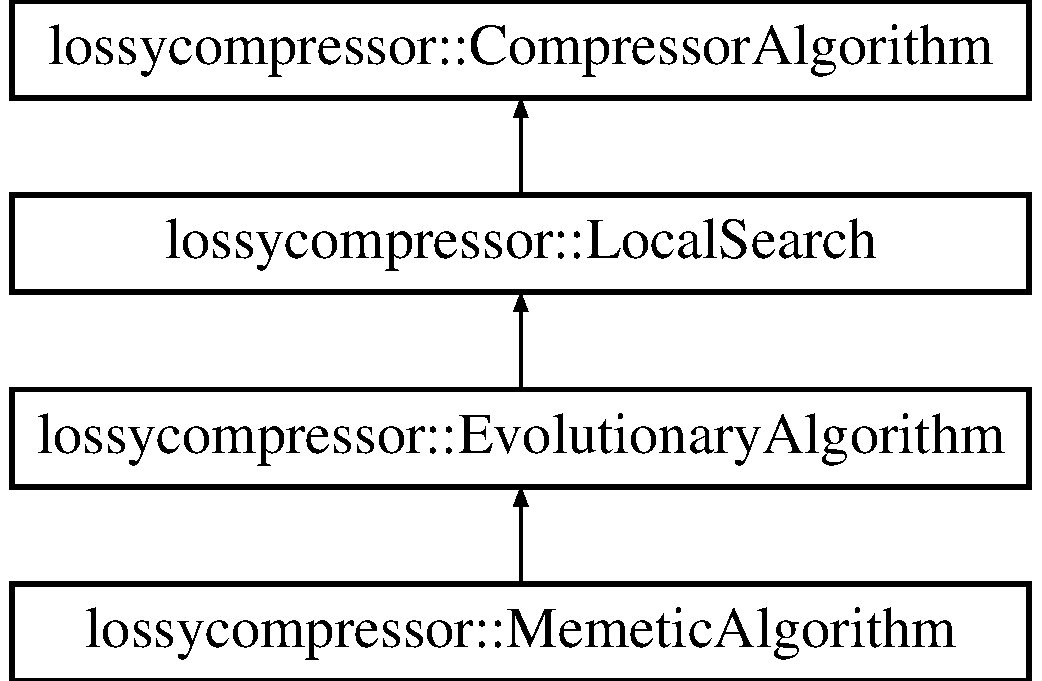
\includegraphics[height=4.000000cm]{classlossycompressor_1_1_compressor_algorithm}
\end{center}
\end{figure}
\subsection*{Classes}
\begin{DoxyCompactItemize}
\item 
struct \hyperlink{structlossycompressor_1_1_compressor_algorithm_1_1_args}{Args}
\begin{DoxyCompactList}\small\item\em Instance of this class is passed as a parameter into \hyperlink{classlossycompressor_1_1_compressor_algorithm}{Compressor\+Algorithm}. Contains compression input data and compression settings. \end{DoxyCompactList}\end{DoxyCompactItemize}
\subsection*{Public Member Functions}
\begin{DoxyCompactItemize}
\item 
\hyperlink{classlossycompressor_1_1_compressor_algorithm_a4b98b46955df2877eb714c36b573faa9}{Compressor\+Algorithm} (\hyperlink{structlossycompressor_1_1_compressor_algorithm_1_1_args}{Compressor\+Algorithm\+::\+Args} $\ast$\hyperlink{classlossycompressor_1_1_compressor_algorithm_a7cec23bc2a41ac35617e21466a2f0c46}{args})\hypertarget{classlossycompressor_1_1_compressor_algorithm_a4b98b46955df2877eb714c36b573faa9}{}\label{classlossycompressor_1_1_compressor_algorithm_a4b98b46955df2877eb714c36b573faa9}

\begin{DoxyCompactList}\small\item\em Construct new Compression\+Algorithm. \end{DoxyCompactList}\item 
int \hyperlink{classlossycompressor_1_1_compressor_algorithm_a651e1dd7ef3df5e46a4aad73a8de4c8d}{compress} (\hyperlink{structlossycompressor_1_1_voronoi_diagram}{Voronoi\+Diagram} $\ast$output\+Diagram, \hyperlink{structlossycompressor_1_1_color24bit}{Color24bit} $\ast$colors, int $\ast$pixel\+Point\+Assignment)
\begin{DoxyCompactList}\small\item\em Do the compression. \end{DoxyCompactList}\end{DoxyCompactItemize}
\subsection*{Protected Member Functions}
\begin{DoxyCompactItemize}
\item 
float \hyperlink{classlossycompressor_1_1_compressor_algorithm_af77bb3da1cfcf14c0bed2aa254c4fbd6}{calculate\+Fitness} (\hyperlink{structlossycompressor_1_1_voronoi_diagram}{Voronoi\+Diagram} $\ast$diagram)
\item 
bool \hyperlink{classlossycompressor_1_1_compressor_algorithm_a978361a0f3a5c36d3a82a6fe1b4c4d00}{can\+Continue\+Computing} ()
\item 
void \hyperlink{classlossycompressor_1_1_compressor_algorithm_ac7ce717ecc67256fbc99d9ab8a0569fe}{on\+Best\+Solution\+Found} (float best\+Fitness)\hypertarget{classlossycompressor_1_1_compressor_algorithm_ac7ce717ecc67256fbc99d9ab8a0569fe}{}\label{classlossycompressor_1_1_compressor_algorithm_ac7ce717ecc67256fbc99d9ab8a0569fe}

\begin{DoxyCompactList}\small\item\em Must be called when computation found the best solution and will terminate. \end{DoxyCompactList}\item 
virtual int \hyperlink{classlossycompressor_1_1_compressor_algorithm_a171b7c408749b37c5526fb6bca9e981e}{compress\+Internal} (\hyperlink{structlossycompressor_1_1_voronoi_diagram}{Voronoi\+Diagram} $\ast$output\+Diagram, \hyperlink{structlossycompressor_1_1_color24bit}{Color24bit} $\ast$colors, int $\ast$pixel\+Point\+Assignment)=0\hypertarget{classlossycompressor_1_1_compressor_algorithm_a171b7c408749b37c5526fb6bca9e981e}{}\label{classlossycompressor_1_1_compressor_algorithm_a171b7c408749b37c5526fb6bca9e981e}

\begin{DoxyCompactList}\small\item\em Implement this method to provide the compression calculation. \end{DoxyCompactList}\end{DoxyCompactItemize}
\subsection*{Protected Attributes}
\begin{DoxyCompactItemize}
\item 
\hyperlink{structlossycompressor_1_1_compressor_algorithm_1_1_args}{Compressor\+Algorithm\+::\+Args} $\ast$ \hyperlink{classlossycompressor_1_1_compressor_algorithm_a7cec23bc2a41ac35617e21466a2f0c46}{args}\hypertarget{classlossycompressor_1_1_compressor_algorithm_a7cec23bc2a41ac35617e21466a2f0c46}{}\label{classlossycompressor_1_1_compressor_algorithm_a7cec23bc2a41ac35617e21466a2f0c46}

\begin{DoxyCompactList}\small\item\em Compression arguments. \end{DoxyCompactList}\item 
\hyperlink{classlossycompressor_1_1_cpu_fitness_evaluator}{Cpu\+Fitness\+Evaluator} $\ast$ \hyperlink{classlossycompressor_1_1_compressor_algorithm_a23c2407260dfc34b4cb74dcf270aaae1}{cpu\+Fitness\+Evaluator}\hypertarget{classlossycompressor_1_1_compressor_algorithm_a23c2407260dfc34b4cb74dcf270aaae1}{}\label{classlossycompressor_1_1_compressor_algorithm_a23c2407260dfc34b4cb74dcf270aaae1}

\begin{DoxyCompactList}\small\item\em Fitness evaluator using C\+PU. \end{DoxyCompactList}\end{DoxyCompactItemize}


\subsection{Detailed Description}
Class representing an algorithm that compresses the image. 

Implementations use local search or various genetic algorithms. Therefore this class contains useful methods used in these implementations.

Points in voronoi diagrams used during calculations are kept sorted according to their horizontal (x) coordinate. This sorting speeds up fitness calculation. Points are initially sorted when diagram is generated and during tweaking only the changed point(s) is/are put to their right place.

B\+E\+W\+A\+RE these utility methods use work variables from the instance of this class and hence cannot be executed in parallel. 

\subsection{Member Function Documentation}
\index{lossycompressor\+::\+Compressor\+Algorithm@{lossycompressor\+::\+Compressor\+Algorithm}!calculate\+Fitness@{calculate\+Fitness}}
\index{calculate\+Fitness@{calculate\+Fitness}!lossycompressor\+::\+Compressor\+Algorithm@{lossycompressor\+::\+Compressor\+Algorithm}}
\subsubsection[{\texorpdfstring{calculate\+Fitness(\+Voronoi\+Diagram $\ast$diagram)}{calculateFitness(VoronoiDiagram *diagram)}}]{\setlength{\rightskip}{0pt plus 5cm}float Compressor\+Algorithm\+::calculate\+Fitness (
\begin{DoxyParamCaption}
\item[{{\bf Voronoi\+Diagram} $\ast$}]{diagram}
\end{DoxyParamCaption}
)\hspace{0.3cm}{\ttfamily [protected]}}\hypertarget{classlossycompressor_1_1_compressor_algorithm_af77bb3da1cfcf14c0bed2aa254c4fbd6}{}\label{classlossycompressor_1_1_compressor_algorithm_af77bb3da1cfcf14c0bed2aa254c4fbd6}
Returned fitness is always $>$= 0 with 0 being the best possible value. \index{lossycompressor\+::\+Compressor\+Algorithm@{lossycompressor\+::\+Compressor\+Algorithm}!can\+Continue\+Computing@{can\+Continue\+Computing}}
\index{can\+Continue\+Computing@{can\+Continue\+Computing}!lossycompressor\+::\+Compressor\+Algorithm@{lossycompressor\+::\+Compressor\+Algorithm}}
\subsubsection[{\texorpdfstring{can\+Continue\+Computing()}{canContinueComputing()}}]{\setlength{\rightskip}{0pt plus 5cm}bool Compressor\+Algorithm\+::can\+Continue\+Computing (
\begin{DoxyParamCaption}
{}
\end{DoxyParamCaption}
)\hspace{0.3cm}{\ttfamily [protected]}}\hypertarget{classlossycompressor_1_1_compressor_algorithm_a978361a0f3a5c36d3a82a6fe1b4c4d00}{}\label{classlossycompressor_1_1_compressor_algorithm_a978361a0f3a5c36d3a82a6fe1b4c4d00}
\begin{DoxyReturn}{Returns}
Returns true if computation can continue given it\textquotesingle{}s limit, false otherwise. 
\end{DoxyReturn}
\index{lossycompressor\+::\+Compressor\+Algorithm@{lossycompressor\+::\+Compressor\+Algorithm}!compress@{compress}}
\index{compress@{compress}!lossycompressor\+::\+Compressor\+Algorithm@{lossycompressor\+::\+Compressor\+Algorithm}}
\subsubsection[{\texorpdfstring{compress(\+Voronoi\+Diagram $\ast$output\+Diagram, Color24bit $\ast$colors, int $\ast$pixel\+Point\+Assignment)}{compress(VoronoiDiagram *outputDiagram, Color24bit *colors, int *pixelPointAssignment)}}]{\setlength{\rightskip}{0pt plus 5cm}int Compressor\+Algorithm\+::compress (
\begin{DoxyParamCaption}
\item[{{\bf Voronoi\+Diagram} $\ast$}]{output\+Diagram, }
\item[{{\bf Color24bit} $\ast$}]{colors, }
\item[{int $\ast$}]{pixel\+Point\+Assignment}
\end{DoxyParamCaption}
)}\hypertarget{classlossycompressor_1_1_compressor_algorithm_a651e1dd7ef3df5e46a4aad73a8de4c8d}{}\label{classlossycompressor_1_1_compressor_algorithm_a651e1dd7ef3df5e46a4aad73a8de4c8d}


Do the compression. 


\begin{DoxyParams}[1]{Parameters}
\mbox{\tt in}  & {\em output\+Diagram} & Diagram into which the compression result will be written. \\
\hline
\mbox{\tt in}  & {\em colors} & Array into which colors of points in diagram will be written. \\
\hline
\mbox{\tt in}  & {\em pixel\+Point\+Assignment} & Array into which indices of closest point for every pixel will be written. \\
\hline
\end{DoxyParams}


The documentation for this class was generated from the following files\+:\begin{DoxyCompactItemize}
\item 
Compressor/compressoralgorithm.\+h\item 
Compressor/compressoralgorithm.\+cpp\end{DoxyCompactItemize}

\hypertarget{classlossycompressor_1_1_compressor_utils}{}\section{lossycompressor\+:\+:Compressor\+Utils Class Reference}
\label{classlossycompressor_1_1_compressor_utils}\index{lossycompressor\+::\+Compressor\+Utils@{lossycompressor\+::\+Compressor\+Utils}}


Contains utility methods used in compression.  




{\ttfamily \#include $<$compressorutils.\+h$>$}

\subsection*{Static Public Member Functions}
\begin{DoxyCompactItemize}
\item 
static void \hyperlink{classlossycompressor_1_1_compressor_utils_a5b0e35fe3f5907d16f354be1ae986cd5}{copy\+Point} (\hyperlink{structlossycompressor_1_1_voronoi_diagram}{Voronoi\+Diagram} $\ast$source, \hyperlink{structlossycompressor_1_1_voronoi_diagram}{Voronoi\+Diagram} $\ast$destination, int index)\hypertarget{classlossycompressor_1_1_compressor_utils_a5b0e35fe3f5907d16f354be1ae986cd5}{}\label{classlossycompressor_1_1_compressor_utils_a5b0e35fe3f5907d16f354be1ae986cd5}

\begin{DoxyCompactList}\small\item\em Copy point on given index from source diagram into the destionation diagram. \end{DoxyCompactList}\item 
static void \hyperlink{classlossycompressor_1_1_compressor_utils_add0142376a99e9c052b6b9abfa4ec750}{copy} (\hyperlink{structlossycompressor_1_1_voronoi_diagram}{Voronoi\+Diagram} $\ast$source, \hyperlink{structlossycompressor_1_1_voronoi_diagram}{Voronoi\+Diagram} $\ast$destination)\hypertarget{classlossycompressor_1_1_compressor_utils_add0142376a99e9c052b6b9abfa4ec750}{}\label{classlossycompressor_1_1_compressor_utils_add0142376a99e9c052b6b9abfa4ec750}

\begin{DoxyCompactList}\small\item\em Copy the source diagram into the destionation diagram. \end{DoxyCompactList}\item 
static void \hyperlink{classlossycompressor_1_1_compressor_utils_a8115bf54770caaa0a345daccd29542c9}{generate\+Random\+Diagram} (\hyperlink{structlossycompressor_1_1_voronoi_diagram}{Voronoi\+Diagram} $\ast$output, int32\+\_\+t source\+Width, int32\+\_\+t source\+Height)\hypertarget{classlossycompressor_1_1_compressor_utils_a8115bf54770caaa0a345daccd29542c9}{}\label{classlossycompressor_1_1_compressor_utils_a8115bf54770caaa0a345daccd29542c9}

\begin{DoxyCompactList}\small\item\em Generates random diagram. \end{DoxyCompactList}\item 
static void \hyperlink{classlossycompressor_1_1_compressor_utils_a06515562c64990788ecba2f071b553e8}{swap} (\hyperlink{structlossycompressor_1_1_voronoi_diagram}{Voronoi\+Diagram} $\ast$$\ast$first, \hyperlink{structlossycompressor_1_1_voronoi_diagram}{Voronoi\+Diagram} $\ast$$\ast$second)\hypertarget{classlossycompressor_1_1_compressor_utils_a06515562c64990788ecba2f071b553e8}{}\label{classlossycompressor_1_1_compressor_utils_a06515562c64990788ecba2f071b553e8}

\begin{DoxyCompactList}\small\item\em Swap two diagrams on given pointers. \end{DoxyCompactList}\item 
static int \hyperlink{classlossycompressor_1_1_compressor_utils_a085da7676dfff941451b92c50359b14b}{compare} (\hyperlink{structlossycompressor_1_1_voronoi_diagram}{Voronoi\+Diagram} $\ast$diagram, int first\+Point\+Index, int second\+Point\+Index)\hypertarget{classlossycompressor_1_1_compressor_utils_a085da7676dfff941451b92c50359b14b}{}\label{classlossycompressor_1_1_compressor_utils_a085da7676dfff941451b92c50359b14b}

\begin{DoxyCompactList}\small\item\em Returns the same values as compare(int32\+\_\+t, int32\+\_\+t, int32\+\_\+t, int32\+\_\+t). \end{DoxyCompactList}\item 
static int \hyperlink{classlossycompressor_1_1_compressor_utils_ae85a980244d3f1b8c15c9552716afcdb}{compare} (int firstX, int firstY, int secondX, int secondY)
\begin{DoxyCompactList}\small\item\em Compare two points on X axis. \end{DoxyCompactList}\end{DoxyCompactItemize}


\subsection{Detailed Description}
Contains utility methods used in compression. 

\subsection{Member Function Documentation}
\index{lossycompressor\+::\+Compressor\+Utils@{lossycompressor\+::\+Compressor\+Utils}!compare@{compare}}
\index{compare@{compare}!lossycompressor\+::\+Compressor\+Utils@{lossycompressor\+::\+Compressor\+Utils}}
\subsubsection[{\texorpdfstring{compare(int first\+X, int first\+Y, int second\+X, int second\+Y)}{compare(int firstX, int firstY, int secondX, int secondY)}}]{\setlength{\rightskip}{0pt plus 5cm}int Compressor\+Utils\+::compare (
\begin{DoxyParamCaption}
\item[{int}]{firstX, }
\item[{int}]{firstY, }
\item[{int}]{secondX, }
\item[{int}]{secondY}
\end{DoxyParamCaption}
)\hspace{0.3cm}{\ttfamily [static]}}\hypertarget{classlossycompressor_1_1_compressor_utils_ae85a980244d3f1b8c15c9552716afcdb}{}\label{classlossycompressor_1_1_compressor_utils_ae85a980244d3f1b8c15c9552716afcdb}


Compare two points on X axis. 

Returns number $<$ 0 if first point x coordinate is smaller than second point\textquotesingle{}s x coordinate or x coordinates are equal and first point\textquotesingle{}s y coordinate is smaller than second point\textquotesingle{}s y coordinate. Returns 0 if points are equal, otherwise returns number $>$ 0. 

The documentation for this class was generated from the following files\+:\begin{DoxyCompactItemize}
\item 
Compressor/compressorutils.\+h\item 
Compressor/compressorutils.\+cpp\end{DoxyCompactItemize}

\hypertarget{classlossycompressor_1_1_cpu_fitness_evaluator}{}\section{lossycompressor\+:\+:Cpu\+Fitness\+Evaluator Class Reference}
\label{classlossycompressor_1_1_cpu_fitness_evaluator}\index{lossycompressor\+::\+Cpu\+Fitness\+Evaluator@{lossycompressor\+::\+Cpu\+Fitness\+Evaluator}}


Calculates fitness using only C\+PU.  




{\ttfamily \#include $<$cpufitnessevaluator.\+h$>$}

Inheritance diagram for lossycompressor\+:\+:Cpu\+Fitness\+Evaluator\+:\begin{figure}[H]
\begin{center}
\leavevmode
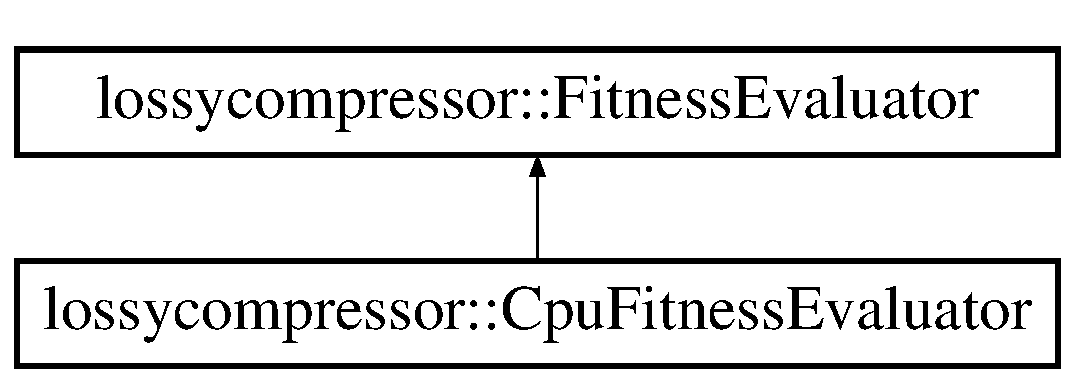
\includegraphics[height=2.000000cm]{classlossycompressor_1_1_cpu_fitness_evaluator}
\end{center}
\end{figure}
\subsection*{Public Member Functions}
\begin{DoxyCompactItemize}
\item 
{\bfseries Cpu\+Fitness\+Evaluator} (int \hyperlink{classlossycompressor_1_1_fitness_evaluator_ab24b1f451eece3d50d030145bdb806f7}{source\+Width}, int \hyperlink{classlossycompressor_1_1_fitness_evaluator_a22151a860849a3b8d0d9d3e2f3b46bdf}{source\+Height}, int \hyperlink{classlossycompressor_1_1_fitness_evaluator_aed694c851ddd4648513cd9c249654272}{diagram\+Points\+Count}, uint8\+\_\+t $\ast$\hyperlink{classlossycompressor_1_1_fitness_evaluator_af75273c5e267ab03a3f3f86c7b043a52}{source\+Image\+Data}, int \hyperlink{classlossycompressor_1_1_fitness_evaluator_a09bd546107e628d4e9e5ff57f078bccf}{source\+Data\+Row\+Width\+In\+Bytes})\hypertarget{classlossycompressor_1_1_cpu_fitness_evaluator_a03c20a21eb4d0680c636111dabb049cb}{}\label{classlossycompressor_1_1_cpu_fitness_evaluator_a03c20a21eb4d0680c636111dabb049cb}

\item 
void \hyperlink{classlossycompressor_1_1_cpu_fitness_evaluator_ad0a6252e1192d086e3734607dbb29b81}{calculate\+Colors} (\hyperlink{structlossycompressor_1_1_voronoi_diagram}{Voronoi\+Diagram} $\ast$diagram, \hyperlink{structlossycompressor_1_1_color24bit}{Color24bit} $\ast$colors, int $\ast$pixel\+Point\+Assignment)\hypertarget{classlossycompressor_1_1_cpu_fitness_evaluator_ad0a6252e1192d086e3734607dbb29b81}{}\label{classlossycompressor_1_1_cpu_fitness_evaluator_ad0a6252e1192d086e3734607dbb29b81}

\begin{DoxyCompactList}\small\item\em Calculates average colors of all points in diagram into the colors array. \end{DoxyCompactList}\end{DoxyCompactItemize}
\subsection*{Protected Member Functions}
\begin{DoxyCompactItemize}
\item 
virtual float \hyperlink{classlossycompressor_1_1_cpu_fitness_evaluator_a96a8323ab453f289d4ab8995ad74a380}{calculate\+Fitness\+Internal} (\hyperlink{structlossycompressor_1_1_voronoi_diagram}{Voronoi\+Diagram} $\ast$diagram)
\begin{DoxyCompactList}\small\item\em Calculates fitness of given diagram. \end{DoxyCompactList}\item 
virtual bool \hyperlink{classlossycompressor_1_1_cpu_fitness_evaluator_a0933b2bd259d2ad6e1bbe2b462df5963}{is\+Cuda} ()\hypertarget{classlossycompressor_1_1_cpu_fitness_evaluator_a0933b2bd259d2ad6e1bbe2b462df5963}{}\label{classlossycompressor_1_1_cpu_fitness_evaluator_a0933b2bd259d2ad6e1bbe2b462df5963}

\begin{DoxyCompactList}\small\item\em Return true if computation of fitness is accelerated by C\+U\+DA. \end{DoxyCompactList}\end{DoxyCompactItemize}
\subsection*{Additional Inherited Members}


\subsection{Detailed Description}
Calculates fitness using only C\+PU. 

\subsection{Member Function Documentation}
\index{lossycompressor\+::\+Cpu\+Fitness\+Evaluator@{lossycompressor\+::\+Cpu\+Fitness\+Evaluator}!calculate\+Fitness\+Internal@{calculate\+Fitness\+Internal}}
\index{calculate\+Fitness\+Internal@{calculate\+Fitness\+Internal}!lossycompressor\+::\+Cpu\+Fitness\+Evaluator@{lossycompressor\+::\+Cpu\+Fitness\+Evaluator}}
\subsubsection[{\texorpdfstring{calculate\+Fitness\+Internal(\+Voronoi\+Diagram $\ast$diagram)}{calculateFitnessInternal(VoronoiDiagram *diagram)}}]{\setlength{\rightskip}{0pt plus 5cm}float Cpu\+Fitness\+Evaluator\+::calculate\+Fitness\+Internal (
\begin{DoxyParamCaption}
\item[{{\bf Voronoi\+Diagram} $\ast$}]{diagram}
\end{DoxyParamCaption}
)\hspace{0.3cm}{\ttfamily [protected]}, {\ttfamily [virtual]}}\hypertarget{classlossycompressor_1_1_cpu_fitness_evaluator_a96a8323ab453f289d4ab8995ad74a380}{}\label{classlossycompressor_1_1_cpu_fitness_evaluator_a96a8323ab453f289d4ab8995ad74a380}


Calculates fitness of given diagram. 

Subclasses must implement this method to provide their way of fitness ccalculation. 

Implements \hyperlink{classlossycompressor_1_1_fitness_evaluator_aa58aa833525109f332c302eb38ee5ec8}{lossycompressor\+::\+Fitness\+Evaluator}.



The documentation for this class was generated from the following files\+:\begin{DoxyCompactItemize}
\item 
Compressor/cpufitnessevaluator.\+h\item 
Compressor/cpufitnessevaluator.\+cpp\end{DoxyCompactItemize}

\hypertarget{classlossycompressor_1_1_cuda_fitness_evaluator}{}\section{lossycompressor\+:\+:Cuda\+Fitness\+Evaluator Class Reference}
\label{classlossycompressor_1_1_cuda_fitness_evaluator}\index{lossycompressor\+::\+Cuda\+Fitness\+Evaluator@{lossycompressor\+::\+Cuda\+Fitness\+Evaluator}}


Calculates fitness. The calculation is accelerated by C\+U\+DA.  




{\ttfamily \#include $<$cudafitnessevaluator.\+h$>$}

Inheritance diagram for lossycompressor\+:\+:Cuda\+Fitness\+Evaluator\+:\begin{figure}[H]
\begin{center}
\leavevmode
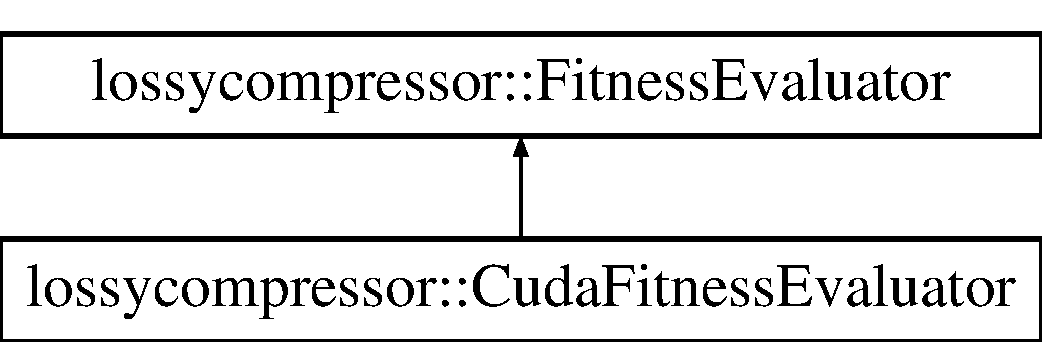
\includegraphics[height=2.000000cm]{classlossycompressor_1_1_cuda_fitness_evaluator}
\end{center}
\end{figure}
\subsection*{Public Member Functions}
\begin{DoxyCompactItemize}
\item 
{\bfseries Cuda\+Fitness\+Evaluator} (int \hyperlink{classlossycompressor_1_1_fitness_evaluator_ab24b1f451eece3d50d030145bdb806f7}{source\+Width}, int \hyperlink{classlossycompressor_1_1_fitness_evaluator_a22151a860849a3b8d0d9d3e2f3b46bdf}{source\+Height}, int \hyperlink{classlossycompressor_1_1_fitness_evaluator_aed694c851ddd4648513cd9c249654272}{diagram\+Points\+Count}, uint8\+\_\+t $\ast$\hyperlink{classlossycompressor_1_1_fitness_evaluator_af75273c5e267ab03a3f3f86c7b043a52}{source\+Image\+Data}, int \hyperlink{classlossycompressor_1_1_fitness_evaluator_a09bd546107e628d4e9e5ff57f078bccf}{source\+Data\+Row\+Width\+In\+Bytes})\hypertarget{classlossycompressor_1_1_cuda_fitness_evaluator_a90dc58cd5a34647f0d90df10fcfea278}{}\label{classlossycompressor_1_1_cuda_fitness_evaluator_a90dc58cd5a34647f0d90df10fcfea278}

\end{DoxyCompactItemize}
\subsection*{Protected Member Functions}
\begin{DoxyCompactItemize}
\item 
virtual float \hyperlink{classlossycompressor_1_1_cuda_fitness_evaluator_a9b0422ff3cd37e1b33ad0fe4478609c1}{calculate\+Fitness\+Internal} (\hyperlink{structlossycompressor_1_1_voronoi_diagram}{Voronoi\+Diagram} $\ast$diagram)
\begin{DoxyCompactList}\small\item\em Calculates fitness of given diagram. \end{DoxyCompactList}\item 
virtual bool \hyperlink{classlossycompressor_1_1_cuda_fitness_evaluator_a71fe5eb07edc8518aa5c1a919d5e143f}{is\+Cuda} ()\hypertarget{classlossycompressor_1_1_cuda_fitness_evaluator_a71fe5eb07edc8518aa5c1a919d5e143f}{}\label{classlossycompressor_1_1_cuda_fitness_evaluator_a71fe5eb07edc8518aa5c1a919d5e143f}

\begin{DoxyCompactList}\small\item\em Return true if computation of fitness is accelerated by C\+U\+DA. \end{DoxyCompactList}\end{DoxyCompactItemize}
\subsection*{Additional Inherited Members}


\subsection{Detailed Description}
Calculates fitness. The calculation is accelerated by C\+U\+DA. 

\subsection{Member Function Documentation}
\index{lossycompressor\+::\+Cuda\+Fitness\+Evaluator@{lossycompressor\+::\+Cuda\+Fitness\+Evaluator}!calculate\+Fitness\+Internal@{calculate\+Fitness\+Internal}}
\index{calculate\+Fitness\+Internal@{calculate\+Fitness\+Internal}!lossycompressor\+::\+Cuda\+Fitness\+Evaluator@{lossycompressor\+::\+Cuda\+Fitness\+Evaluator}}
\subsubsection[{\texorpdfstring{calculate\+Fitness\+Internal(\+Voronoi\+Diagram $\ast$diagram)}{calculateFitnessInternal(VoronoiDiagram *diagram)}}]{\setlength{\rightskip}{0pt plus 5cm}virtual float lossycompressor\+::\+Cuda\+Fitness\+Evaluator\+::calculate\+Fitness\+Internal (
\begin{DoxyParamCaption}
\item[{{\bf Voronoi\+Diagram} $\ast$}]{diagram}
\end{DoxyParamCaption}
)\hspace{0.3cm}{\ttfamily [protected]}, {\ttfamily [virtual]}}\hypertarget{classlossycompressor_1_1_cuda_fitness_evaluator_a9b0422ff3cd37e1b33ad0fe4478609c1}{}\label{classlossycompressor_1_1_cuda_fitness_evaluator_a9b0422ff3cd37e1b33ad0fe4478609c1}


Calculates fitness of given diagram. 

Subclasses must implement this method to provide their way of fitness ccalculation. 

Implements \hyperlink{classlossycompressor_1_1_fitness_evaluator_aa58aa833525109f332c302eb38ee5ec8}{lossycompressor\+::\+Fitness\+Evaluator}.



The documentation for this class was generated from the following file\+:\begin{DoxyCompactItemize}
\item 
Compressor/cudafitnessevaluator.\+h\end{DoxyCompactItemize}

\hypertarget{classlossycompressor_1_1_evolutionary_algorithm}{}\section{lossycompressor\+:\+:Evolutionary\+Algorithm Class Reference}
\label{classlossycompressor_1_1_evolutionary_algorithm}\index{lossycompressor\+::\+Evolutionary\+Algorithm@{lossycompressor\+::\+Evolutionary\+Algorithm}}


Uses evolutionary algorithm to come up with best position of diagram points.  




{\ttfamily \#include $<$evolutionaryalgorithm.\+h$>$}

Inheritance diagram for lossycompressor\+:\+:Evolutionary\+Algorithm\+:\begin{figure}[H]
\begin{center}
\leavevmode
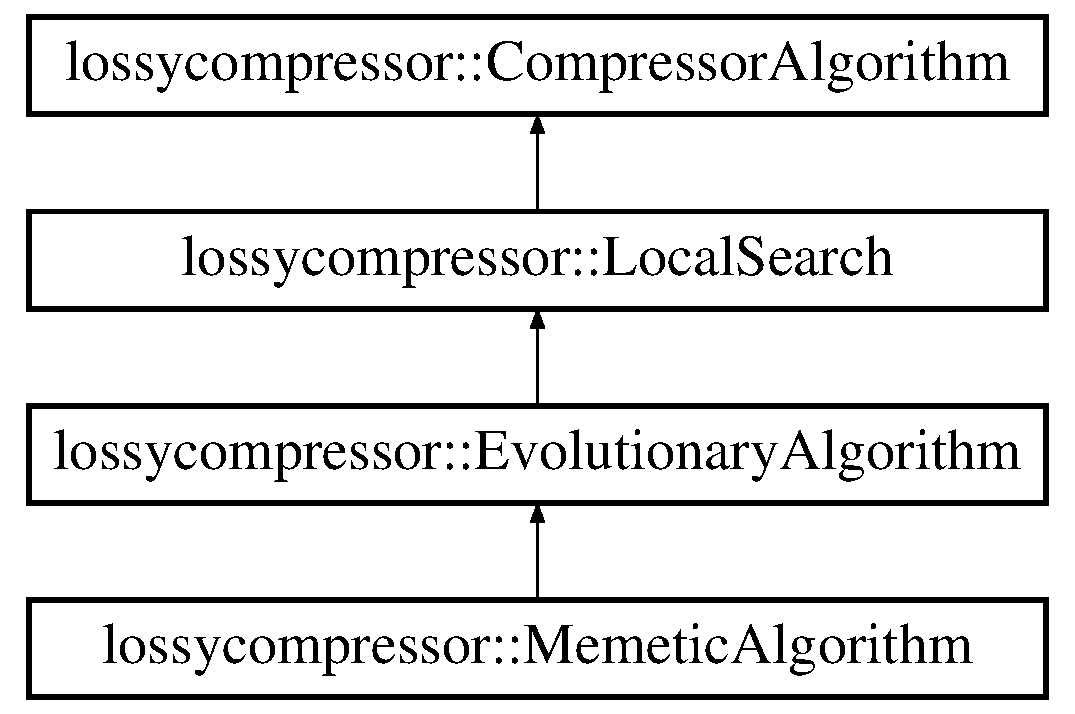
\includegraphics[height=4.000000cm]{classlossycompressor_1_1_evolutionary_algorithm}
\end{center}
\end{figure}
\subsection*{Public Member Functions}
\begin{DoxyCompactItemize}
\item 
{\bfseries Evolutionary\+Algorithm} (\hyperlink{structlossycompressor_1_1_compressor_algorithm_1_1_args}{Compressor\+Algorithm\+::\+Args} $\ast$\hyperlink{classlossycompressor_1_1_compressor_algorithm_a7cec23bc2a41ac35617e21466a2f0c46}{args})\hypertarget{classlossycompressor_1_1_evolutionary_algorithm_a145e42ac3f5b468dace534257e24196a}{}\label{classlossycompressor_1_1_evolutionary_algorithm_a145e42ac3f5b468dace534257e24196a}

\end{DoxyCompactItemize}
\subsection*{Protected Member Functions}
\begin{DoxyCompactItemize}
\item 
void \hyperlink{classlossycompressor_1_1_evolutionary_algorithm_a212ab81cd050216479830b18d93ca853}{crossover} (\hyperlink{structlossycompressor_1_1_voronoi_diagram}{Voronoi\+Diagram} $\ast$first\+Parent, \hyperlink{structlossycompressor_1_1_voronoi_diagram}{Voronoi\+Diagram} $\ast$second\+Parent, \hyperlink{structlossycompressor_1_1_voronoi_diagram}{Voronoi\+Diagram} $\ast$first\+Child, \hyperlink{structlossycompressor_1_1_voronoi_diagram}{Voronoi\+Diagram} $\ast$second\+Child)\hypertarget{classlossycompressor_1_1_evolutionary_algorithm_a212ab81cd050216479830b18d93ca853}{}\label{classlossycompressor_1_1_evolutionary_algorithm_a212ab81cd050216479830b18d93ca853}

\begin{DoxyCompactList}\small\item\em Does crossover of given parents and stores the results into given children. \end{DoxyCompactList}\item 
void \hyperlink{classlossycompressor_1_1_evolutionary_algorithm_ad58c5cbe04826032c5b5ba86f3db9aa1}{generate\+Initial\+Population} (int population\+Size, vector$<$ \hyperlink{structlossycompressor_1_1_voronoi_diagram}{Voronoi\+Diagram} $\ast$ $>$ $\ast$population, vector$<$ float $>$ $\ast$population\+Fitness, float $\ast$best\+Fitness, \hyperlink{structlossycompressor_1_1_voronoi_diagram}{Voronoi\+Diagram} $\ast$$\ast$best)
\begin{DoxyCompactList}\small\item\em Generates initial population. \end{DoxyCompactList}\item 
void \hyperlink{classlossycompressor_1_1_evolutionary_algorithm_a9e97a1b8ad2befd1e42e28fd348062c2}{selection} (int selection\+Size, vector$<$ \hyperlink{structlossycompressor_1_1_voronoi_diagram}{Voronoi\+Diagram} $\ast$ $>$ $\ast$population, vector$<$ float $>$ $\ast$population\+Fitness, vector$<$ \hyperlink{structlossycompressor_1_1_voronoi_diagram}{Voronoi\+Diagram} $\ast$ $>$ $\ast$diagram\+Pool)\hypertarget{classlossycompressor_1_1_evolutionary_algorithm_a9e97a1b8ad2befd1e42e28fd348062c2}{}\label{classlossycompressor_1_1_evolutionary_algorithm_a9e97a1b8ad2befd1e42e28fd348062c2}

\begin{DoxyCompactList}\small\item\em Does selection on given population. \end{DoxyCompactList}\item 
void \hyperlink{classlossycompressor_1_1_evolutionary_algorithm_ab6bdef7eff196720ed733561e1589411}{breeding} (int breeding\+Size, int max\+Bred\+Member\+Index, vector$<$ \hyperlink{structlossycompressor_1_1_voronoi_diagram}{Voronoi\+Diagram} $\ast$ $>$ $\ast$population, vector$<$ float $>$ $\ast$population\+Fitness, vector$<$ \hyperlink{structlossycompressor_1_1_voronoi_diagram}{Voronoi\+Diagram} $\ast$ $>$ $\ast$diagram\+Pool, float $\ast$best\+Fitness, \hyperlink{structlossycompressor_1_1_voronoi_diagram}{Voronoi\+Diagram} $\ast$$\ast$best)\hypertarget{classlossycompressor_1_1_evolutionary_algorithm_ab6bdef7eff196720ed733561e1589411}{}\label{classlossycompressor_1_1_evolutionary_algorithm_ab6bdef7eff196720ed733561e1589411}

\begin{DoxyCompactList}\small\item\em Does breeding on given population. \end{DoxyCompactList}\item 
void \hyperlink{classlossycompressor_1_1_evolutionary_algorithm_ad4a888519faba7e6fb34e237b6b8672a}{mutation} (int mutation\+Size, int max\+Mutated\+Member\+Index, vector$<$ \hyperlink{structlossycompressor_1_1_voronoi_diagram}{Voronoi\+Diagram} $\ast$ $>$ $\ast$population, vector$<$ float $>$ $\ast$population\+Fitness, vector$<$ \hyperlink{structlossycompressor_1_1_voronoi_diagram}{Voronoi\+Diagram} $\ast$ $>$ $\ast$diagram\+Pool, float $\ast$best\+Fitness, \hyperlink{structlossycompressor_1_1_voronoi_diagram}{Voronoi\+Diagram} $\ast$$\ast$best)\hypertarget{classlossycompressor_1_1_evolutionary_algorithm_ad4a888519faba7e6fb34e237b6b8672a}{}\label{classlossycompressor_1_1_evolutionary_algorithm_ad4a888519faba7e6fb34e237b6b8672a}

\begin{DoxyCompactList}\small\item\em Mutates mutation\+Size new members from current population. Shuffles the population so that same member is not mutated twice. \end{DoxyCompactList}\item 
virtual int \hyperlink{classlossycompressor_1_1_evolutionary_algorithm_a9fcfb7a87adc89ea05046ae9b352c64c}{compress\+Internal} (\hyperlink{structlossycompressor_1_1_voronoi_diagram}{Voronoi\+Diagram} $\ast$output\+Diagram, \hyperlink{structlossycompressor_1_1_color24bit}{Color24bit} $\ast$colors, int $\ast$pixel\+Point\+Assignment) override\hypertarget{classlossycompressor_1_1_evolutionary_algorithm_a9fcfb7a87adc89ea05046ae9b352c64c}{}\label{classlossycompressor_1_1_evolutionary_algorithm_a9fcfb7a87adc89ea05046ae9b352c64c}

\begin{DoxyCompactList}\small\item\em Implement this method to provide the compression calculation. \end{DoxyCompactList}\end{DoxyCompactItemize}
\subsection*{Additional Inherited Members}


\subsection{Detailed Description}
Uses evolutionary algorithm to come up with best position of diagram points. 

\subsection{Member Function Documentation}
\index{lossycompressor\+::\+Evolutionary\+Algorithm@{lossycompressor\+::\+Evolutionary\+Algorithm}!generate\+Initial\+Population@{generate\+Initial\+Population}}
\index{generate\+Initial\+Population@{generate\+Initial\+Population}!lossycompressor\+::\+Evolutionary\+Algorithm@{lossycompressor\+::\+Evolutionary\+Algorithm}}
\subsubsection[{\texorpdfstring{generate\+Initial\+Population(int population\+Size, vector$<$ Voronoi\+Diagram $\ast$ $>$ $\ast$population, vector$<$ float $>$ $\ast$population\+Fitness, float $\ast$best\+Fitness, Voronoi\+Diagram $\ast$$\ast$best)}{generateInitialPopulation(int populationSize, vector< VoronoiDiagram * > *population, vector< float > *populationFitness, float *bestFitness, VoronoiDiagram **best)}}]{\setlength{\rightskip}{0pt plus 5cm}void Evolutionary\+Algorithm\+::generate\+Initial\+Population (
\begin{DoxyParamCaption}
\item[{int}]{population\+Size, }
\item[{vector$<$ {\bf Voronoi\+Diagram} $\ast$ $>$ $\ast$}]{population, }
\item[{vector$<$ float $>$ $\ast$}]{population\+Fitness, }
\item[{float $\ast$}]{best\+Fitness, }
\item[{{\bf Voronoi\+Diagram} $\ast$$\ast$}]{best}
\end{DoxyParamCaption}
)\hspace{0.3cm}{\ttfamily [protected]}}\hypertarget{classlossycompressor_1_1_evolutionary_algorithm_ad58c5cbe04826032c5b5ba86f3db9aa1}{}\label{classlossycompressor_1_1_evolutionary_algorithm_ad58c5cbe04826032c5b5ba86f3db9aa1}


Generates initial population. 

/param\mbox{[}in\mbox{]} population\+Size Size of the initial population. /param\mbox{[}out\mbox{]} population Vector into which the generated population will be stored. /param\mbox{[}out\mbox{]} population\+Fitness Vector in which fitness values of population members will be stored. /param\mbox{[}out\mbox{]} best\+Fitness On location of this pointer the fitness of best population member will be stored. /param\mbox{[}out\mbox{]} best Into the pointer referenced by this variable best population member will be stored. 

The documentation for this class was generated from the following files\+:\begin{DoxyCompactItemize}
\item 
Compressor/evolutionaryalgorithm.\+h\item 
Compressor/evolutionaryalgorithm.\+cpp\end{DoxyCompactItemize}

\hypertarget{classlossycompressor_1_1_fitness_evaluator}{}\section{lossycompressor\+:\+:Fitness\+Evaluator Class Reference}
\label{classlossycompressor_1_1_fitness_evaluator}\index{lossycompressor\+::\+Fitness\+Evaluator@{lossycompressor\+::\+Fitness\+Evaluator}}


Base class for fitness evaluator. Subclasses must provide concrete fitness calculation methods.  




{\ttfamily \#include $<$fitnessevaluator.\+h$>$}

Inheritance diagram for lossycompressor\+:\+:Fitness\+Evaluator\+:\begin{figure}[H]
\begin{center}
\leavevmode
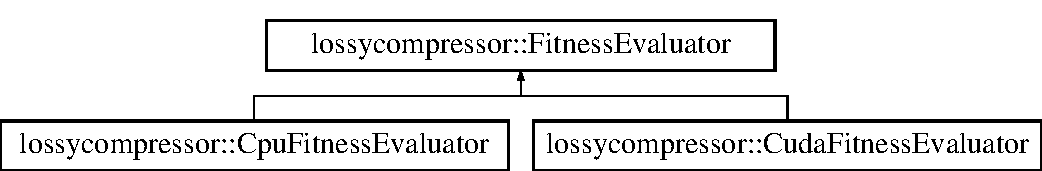
\includegraphics[height=2.000000cm]{classlossycompressor_1_1_fitness_evaluator}
\end{center}
\end{figure}
\subsection*{Public Member Functions}
\begin{DoxyCompactItemize}
\item 
\hyperlink{classlossycompressor_1_1_fitness_evaluator_a323cb74e5d3d02d779b91facf1cc2723}{Fitness\+Evaluator} (int \hyperlink{classlossycompressor_1_1_fitness_evaluator_ab24b1f451eece3d50d030145bdb806f7}{source\+Width}, int \hyperlink{classlossycompressor_1_1_fitness_evaluator_a22151a860849a3b8d0d9d3e2f3b46bdf}{source\+Height}, int \hyperlink{classlossycompressor_1_1_fitness_evaluator_aed694c851ddd4648513cd9c249654272}{diagram\+Points\+Count}, uint8\+\_\+t $\ast$\hyperlink{classlossycompressor_1_1_fitness_evaluator_af75273c5e267ab03a3f3f86c7b043a52}{source\+Image\+Data}, int \hyperlink{classlossycompressor_1_1_fitness_evaluator_a09bd546107e628d4e9e5ff57f078bccf}{source\+Data\+Row\+Width\+In\+Bytes})\hypertarget{classlossycompressor_1_1_fitness_evaluator_a323cb74e5d3d02d779b91facf1cc2723}{}\label{classlossycompressor_1_1_fitness_evaluator_a323cb74e5d3d02d779b91facf1cc2723}

\begin{DoxyCompactList}\small\item\em Construct a new \hyperlink{classlossycompressor_1_1_fitness_evaluator}{Fitness\+Evaluator}. \end{DoxyCompactList}\item 
float \hyperlink{classlossycompressor_1_1_fitness_evaluator_a5b469667f1d70ccb2b4326c9627fea40}{calculate\+Fitness} (\hyperlink{structlossycompressor_1_1_voronoi_diagram}{Voronoi\+Diagram} $\ast$diagram)\hypertarget{classlossycompressor_1_1_fitness_evaluator_a5b469667f1d70ccb2b4326c9627fea40}{}\label{classlossycompressor_1_1_fitness_evaluator_a5b469667f1d70ccb2b4326c9627fea40}

\begin{DoxyCompactList}\small\item\em Calculates fitness of given diagram. \end{DoxyCompactList}\item 
int \hyperlink{classlossycompressor_1_1_fitness_evaluator_af96a4665f6e6041e06d7db2771efb9ac}{get\+Fitness\+Evaluations\+Count} ()\hypertarget{classlossycompressor_1_1_fitness_evaluator_af96a4665f6e6041e06d7db2771efb9ac}{}\label{classlossycompressor_1_1_fitness_evaluator_af96a4665f6e6041e06d7db2771efb9ac}

\begin{DoxyCompactList}\small\item\em Returns count of fitness evaluations done by this evaluator. \end{DoxyCompactList}\item 
void \hyperlink{classlossycompressor_1_1_fitness_evaluator_a9251ae55a79031d6bcffbe7dbff34d31}{reset\+Fitness\+Calculation\+Count} ()\hypertarget{classlossycompressor_1_1_fitness_evaluator_a9251ae55a79031d6bcffbe7dbff34d31}{}\label{classlossycompressor_1_1_fitness_evaluator_a9251ae55a79031d6bcffbe7dbff34d31}

\begin{DoxyCompactList}\small\item\em Resets the fitness evaluations count. \end{DoxyCompactList}\end{DoxyCompactItemize}
\subsection*{Protected Member Functions}
\begin{DoxyCompactItemize}
\item 
virtual float \hyperlink{classlossycompressor_1_1_fitness_evaluator_aa58aa833525109f332c302eb38ee5ec8}{calculate\+Fitness\+Internal} (\hyperlink{structlossycompressor_1_1_voronoi_diagram}{Voronoi\+Diagram} $\ast$diagram)=0
\begin{DoxyCompactList}\small\item\em Calculates fitness of given diagram. \end{DoxyCompactList}\item 
virtual bool \hyperlink{classlossycompressor_1_1_fitness_evaluator_a8112713ec4397ed2d83d3fd6f5b15895}{is\+Cuda} ()=0\hypertarget{classlossycompressor_1_1_fitness_evaluator_a8112713ec4397ed2d83d3fd6f5b15895}{}\label{classlossycompressor_1_1_fitness_evaluator_a8112713ec4397ed2d83d3fd6f5b15895}

\begin{DoxyCompactList}\small\item\em Return true if computation of fitness is accelerated by C\+U\+DA. \end{DoxyCompactList}\end{DoxyCompactItemize}
\subsection*{Protected Attributes}
\begin{DoxyCompactItemize}
\item 
int \hyperlink{classlossycompressor_1_1_fitness_evaluator_ab24b1f451eece3d50d030145bdb806f7}{source\+Width}\hypertarget{classlossycompressor_1_1_fitness_evaluator_ab24b1f451eece3d50d030145bdb806f7}{}\label{classlossycompressor_1_1_fitness_evaluator_ab24b1f451eece3d50d030145bdb806f7}

\begin{DoxyCompactList}\small\item\em Width of source image. \end{DoxyCompactList}\item 
int \hyperlink{classlossycompressor_1_1_fitness_evaluator_a22151a860849a3b8d0d9d3e2f3b46bdf}{source\+Height}\hypertarget{classlossycompressor_1_1_fitness_evaluator_a22151a860849a3b8d0d9d3e2f3b46bdf}{}\label{classlossycompressor_1_1_fitness_evaluator_a22151a860849a3b8d0d9d3e2f3b46bdf}

\begin{DoxyCompactList}\small\item\em Height of source image. \end{DoxyCompactList}\item 
int \hyperlink{classlossycompressor_1_1_fitness_evaluator_aed694c851ddd4648513cd9c249654272}{diagram\+Points\+Count}\hypertarget{classlossycompressor_1_1_fitness_evaluator_aed694c851ddd4648513cd9c249654272}{}\label{classlossycompressor_1_1_fitness_evaluator_aed694c851ddd4648513cd9c249654272}

\begin{DoxyCompactList}\small\item\em Count of points in diagram. \end{DoxyCompactList}\item 
uint8\+\_\+t $\ast$ \hyperlink{classlossycompressor_1_1_fitness_evaluator_af75273c5e267ab03a3f3f86c7b043a52}{source\+Image\+Data}\hypertarget{classlossycompressor_1_1_fitness_evaluator_af75273c5e267ab03a3f3f86c7b043a52}{}\label{classlossycompressor_1_1_fitness_evaluator_af75273c5e267ab03a3f3f86c7b043a52}

\begin{DoxyCompactList}\small\item\em Data of source image. \end{DoxyCompactList}\item 
int \hyperlink{classlossycompressor_1_1_fitness_evaluator_a09bd546107e628d4e9e5ff57f078bccf}{source\+Data\+Row\+Width\+In\+Bytes}\hypertarget{classlossycompressor_1_1_fitness_evaluator_a09bd546107e628d4e9e5ff57f078bccf}{}\label{classlossycompressor_1_1_fitness_evaluator_a09bd546107e628d4e9e5ff57f078bccf}

\begin{DoxyCompactList}\small\item\em Length of a row in source image data. \end{DoxyCompactList}\end{DoxyCompactItemize}


\subsection{Detailed Description}
Base class for fitness evaluator. Subclasses must provide concrete fitness calculation methods. 

\subsection{Member Function Documentation}
\index{lossycompressor\+::\+Fitness\+Evaluator@{lossycompressor\+::\+Fitness\+Evaluator}!calculate\+Fitness\+Internal@{calculate\+Fitness\+Internal}}
\index{calculate\+Fitness\+Internal@{calculate\+Fitness\+Internal}!lossycompressor\+::\+Fitness\+Evaluator@{lossycompressor\+::\+Fitness\+Evaluator}}
\subsubsection[{\texorpdfstring{calculate\+Fitness\+Internal(\+Voronoi\+Diagram $\ast$diagram)=0}{calculateFitnessInternal(VoronoiDiagram *diagram)=0}}]{\setlength{\rightskip}{0pt plus 5cm}virtual float lossycompressor\+::\+Fitness\+Evaluator\+::calculate\+Fitness\+Internal (
\begin{DoxyParamCaption}
\item[{{\bf Voronoi\+Diagram} $\ast$}]{diagram}
\end{DoxyParamCaption}
)\hspace{0.3cm}{\ttfamily [protected]}, {\ttfamily [pure virtual]}}\hypertarget{classlossycompressor_1_1_fitness_evaluator_aa58aa833525109f332c302eb38ee5ec8}{}\label{classlossycompressor_1_1_fitness_evaluator_aa58aa833525109f332c302eb38ee5ec8}


Calculates fitness of given diagram. 

Subclasses must implement this method to provide their way of fitness ccalculation. 

Implemented in \hyperlink{classlossycompressor_1_1_cpu_fitness_evaluator_a96a8323ab453f289d4ab8995ad74a380}{lossycompressor\+::\+Cpu\+Fitness\+Evaluator}, and \hyperlink{classlossycompressor_1_1_cuda_fitness_evaluator_a9b0422ff3cd37e1b33ad0fe4478609c1}{lossycompressor\+::\+Cuda\+Fitness\+Evaluator}.



The documentation for this class was generated from the following files\+:\begin{DoxyCompactItemize}
\item 
Compressor/fitnessevaluator.\+h\item 
Compressor/fitnessevaluator.\+cpp\end{DoxyCompactItemize}

\hypertarget{classlossycompressor_1_1_local_search}{}\section{lossycompressor\+:\+:Local\+Search Class Reference}
\label{classlossycompressor_1_1_local_search}\index{lossycompressor\+::\+Local\+Search@{lossycompressor\+::\+Local\+Search}}


Uses hill-\/climbing to come up with best position of diagram points.  




{\ttfamily \#include $<$localsearch.\+h$>$}

Inheritance diagram for lossycompressor\+:\+:Local\+Search\+:\begin{figure}[H]
\begin{center}
\leavevmode
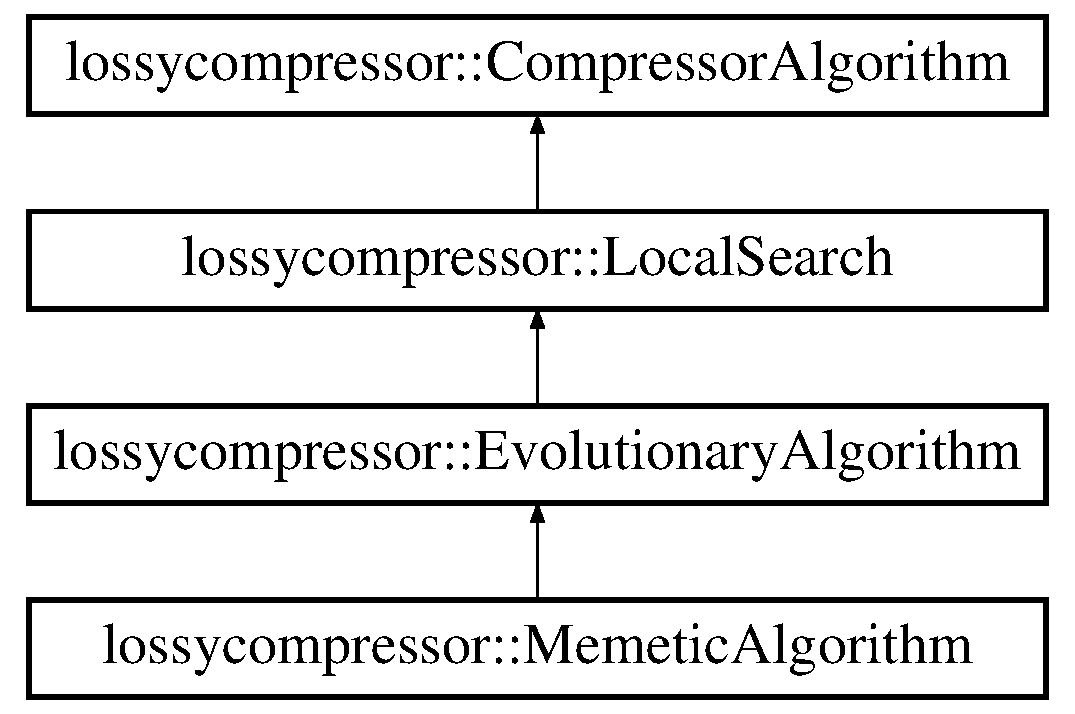
\includegraphics[height=4.000000cm]{classlossycompressor_1_1_local_search}
\end{center}
\end{figure}
\subsection*{Public Member Functions}
\begin{DoxyCompactItemize}
\item 
{\bfseries Local\+Search} (\hyperlink{structlossycompressor_1_1_compressor_algorithm_1_1_args}{Compressor\+Algorithm\+::\+Args} $\ast$\hyperlink{classlossycompressor_1_1_compressor_algorithm_a7cec23bc2a41ac35617e21466a2f0c46}{args})\hypertarget{classlossycompressor_1_1_local_search_a485d8d669395cf70638829f24dacea40}{}\label{classlossycompressor_1_1_local_search_a485d8d669395cf70638829f24dacea40}

\end{DoxyCompactItemize}
\subsection*{Protected Member Functions}
\begin{DoxyCompactItemize}
\item 
void \hyperlink{classlossycompressor_1_1_local_search_a3531b177402f98c172e412333310ec58}{tweak} (\hyperlink{structlossycompressor_1_1_voronoi_diagram}{Voronoi\+Diagram} $\ast$source, \hyperlink{structlossycompressor_1_1_voronoi_diagram}{Voronoi\+Diagram} $\ast$destination)\hypertarget{classlossycompressor_1_1_local_search_a3531b177402f98c172e412333310ec58}{}\label{classlossycompressor_1_1_local_search_a3531b177402f98c172e412333310ec58}

\begin{DoxyCompactList}\small\item\em Tweaks the source diagram and copies it into destination diagram. \end{DoxyCompactList}\item 
virtual int \hyperlink{classlossycompressor_1_1_local_search_a23f2fb30df43d1166c1a2340e79cda06}{compress\+Internal} (\hyperlink{structlossycompressor_1_1_voronoi_diagram}{Voronoi\+Diagram} $\ast$output\+Diagram, \hyperlink{structlossycompressor_1_1_color24bit}{Color24bit} $\ast$colors, int $\ast$pixel\+Point\+Assignment) override\hypertarget{classlossycompressor_1_1_local_search_a23f2fb30df43d1166c1a2340e79cda06}{}\label{classlossycompressor_1_1_local_search_a23f2fb30df43d1166c1a2340e79cda06}

\begin{DoxyCompactList}\small\item\em Implement this method to provide the compression calculation. \end{DoxyCompactList}\end{DoxyCompactItemize}
\subsection*{Additional Inherited Members}


\subsection{Detailed Description}
Uses hill-\/climbing to come up with best position of diagram points. 

The documentation for this class was generated from the following files\+:\begin{DoxyCompactItemize}
\item 
Compressor/localsearch.\+h\item 
Compressor/localsearch.\+cpp\end{DoxyCompactItemize}

\hypertarget{classlossycompressor_1_1_memetic_algorithm}{}\section{lossycompressor\+:\+:Memetic\+Algorithm Class Reference}
\label{classlossycompressor_1_1_memetic_algorithm}\index{lossycompressor\+::\+Memetic\+Algorithm@{lossycompressor\+::\+Memetic\+Algorithm}}


Uses memetic algorithm to come up with best position of diagram points.  




{\ttfamily \#include $<$memeticalgorithm.\+h$>$}

Inheritance diagram for lossycompressor\+:\+:Memetic\+Algorithm\+:\begin{figure}[H]
\begin{center}
\leavevmode
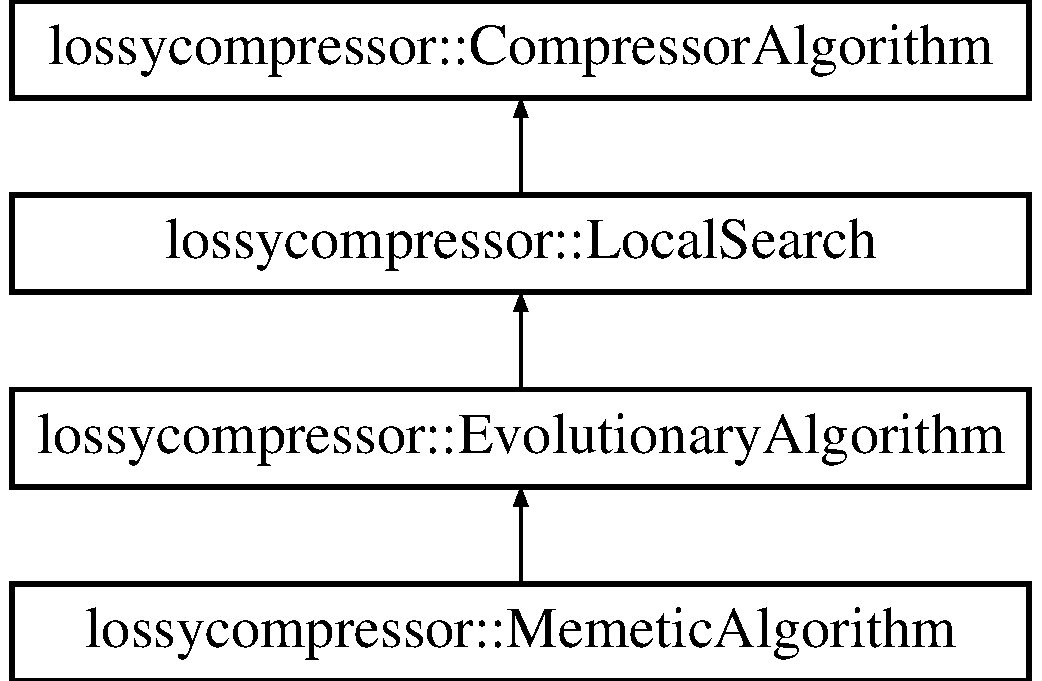
\includegraphics[height=4.000000cm]{classlossycompressor_1_1_memetic_algorithm}
\end{center}
\end{figure}
\subsection*{Public Member Functions}
\begin{DoxyCompactItemize}
\item 
{\bfseries Memetic\+Algorithm} (\hyperlink{structlossycompressor_1_1_compressor_algorithm_1_1_args}{Compressor\+Algorithm\+::\+Args} $\ast$\hyperlink{classlossycompressor_1_1_compressor_algorithm_a7cec23bc2a41ac35617e21466a2f0c46}{args})\hypertarget{classlossycompressor_1_1_memetic_algorithm_a5cef9ea6d77bb7ec8f5864d39c2215cc}{}\label{classlossycompressor_1_1_memetic_algorithm_a5cef9ea6d77bb7ec8f5864d39c2215cc}

\end{DoxyCompactItemize}
\subsection*{Protected Member Functions}
\begin{DoxyCompactItemize}
\item 
virtual int \hyperlink{classlossycompressor_1_1_memetic_algorithm_a04b6e6ac9468808694b006f283d1e6d9}{compress\+Internal} (\hyperlink{structlossycompressor_1_1_voronoi_diagram}{Voronoi\+Diagram} $\ast$output\+Diagram, \hyperlink{structlossycompressor_1_1_color24bit}{Color24bit} $\ast$colors, int $\ast$pixel\+Point\+Assignment) override\hypertarget{classlossycompressor_1_1_memetic_algorithm_a04b6e6ac9468808694b006f283d1e6d9}{}\label{classlossycompressor_1_1_memetic_algorithm_a04b6e6ac9468808694b006f283d1e6d9}

\begin{DoxyCompactList}\small\item\em Implement this method to provide the compression calculation. \end{DoxyCompactList}\end{DoxyCompactItemize}
\subsection*{Additional Inherited Members}


\subsection{Detailed Description}
Uses memetic algorithm to come up with best position of diagram points. 

The documentation for this class was generated from the following files\+:\begin{DoxyCompactItemize}
\item 
Compressor/memeticalgorithm.\+h\item 
Compressor/memeticalgorithm.\+cpp\end{DoxyCompactItemize}

\hypertarget{classlossycompressor_1_1_utils}{}\section{lossycompressor\+:\+:Utils Class Reference}
\label{classlossycompressor_1_1_utils}\index{lossycompressor\+::\+Utils@{lossycompressor\+::\+Utils}}


Contains general utility methods.  




{\ttfamily \#include $<$utils.\+h$>$}

\subsection*{Static Public Member Functions}
\begin{DoxyCompactItemize}
\item 
static void \hyperlink{classlossycompressor_1_1_utils_a23beba13407961e8db9a9efac0b8780f}{swap} (int32\+\_\+t $\ast$arr, int first\+Index, int second\+Index)\hypertarget{classlossycompressor_1_1_utils_a23beba13407961e8db9a9efac0b8780f}{}\label{classlossycompressor_1_1_utils_a23beba13407961e8db9a9efac0b8780f}

\begin{DoxyCompactList}\small\item\em Swap two data items in an array. \end{DoxyCompactList}\item 
static int \hyperlink{classlossycompressor_1_1_utils_adf879284f3bd313d718228dba638a81b}{max} (int first, int second)\hypertarget{classlossycompressor_1_1_utils_adf879284f3bd313d718228dba638a81b}{}\label{classlossycompressor_1_1_utils_adf879284f3bd313d718228dba638a81b}

\begin{DoxyCompactList}\small\item\em Return the greater value out of the two argument. \end{DoxyCompactList}\item 
static double \hyperlink{classlossycompressor_1_1_utils_a3d136b63cc748174616feefd2340dcab}{calculate\+Square\+Distance} (int firstX, int firstY, int secondX, int secondY)
\begin{DoxyCompactList}\small\item\em Calculate squared distance between the two points. \end{DoxyCompactList}\item 
static void \hyperlink{classlossycompressor_1_1_utils_a43e36268d9b4f77989190d5a7b36485c}{record\+Time} (L\+A\+R\+G\+E\+\_\+\+I\+N\+T\+E\+G\+ER $\ast$event)
\begin{DoxyCompactList}\small\item\em Record current time using the Windows A\+PI. \end{DoxyCompactList}\item 
static double \hyperlink{classlossycompressor_1_1_utils_a1b60e219b809c694aa9ca980288fc618}{calculate\+Interval} (L\+A\+R\+G\+E\+\_\+\+I\+N\+T\+E\+G\+ER $\ast$start, L\+A\+R\+G\+E\+\_\+\+I\+N\+T\+E\+G\+ER $\ast$end)\hypertarget{classlossycompressor_1_1_utils_a1b60e219b809c694aa9ca980288fc618}{}\label{classlossycompressor_1_1_utils_a1b60e219b809c694aa9ca980288fc618}

\begin{DoxyCompactList}\small\item\em Calculate time interval between two events. \end{DoxyCompactList}\item 
static int \hyperlink{classlossycompressor_1_1_utils_a906f479a554b2b819d6116155b3efb1d}{generate\+Random} (int \hyperlink{classlossycompressor_1_1_utils_adf879284f3bd313d718228dba638a81b}{max})\hypertarget{classlossycompressor_1_1_utils_a906f479a554b2b819d6116155b3efb1d}{}\label{classlossycompressor_1_1_utils_a906f479a554b2b819d6116155b3efb1d}

\begin{DoxyCompactList}\small\item\em Generate random integer between and max inclusive. \end{DoxyCompactList}\end{DoxyCompactItemize}


\subsection{Detailed Description}
Contains general utility methods. 

\subsection{Member Function Documentation}
\index{lossycompressor\+::\+Utils@{lossycompressor\+::\+Utils}!calculate\+Square\+Distance@{calculate\+Square\+Distance}}
\index{calculate\+Square\+Distance@{calculate\+Square\+Distance}!lossycompressor\+::\+Utils@{lossycompressor\+::\+Utils}}
\subsubsection[{\texorpdfstring{calculate\+Square\+Distance(int first\+X, int first\+Y, int second\+X, int second\+Y)}{calculateSquareDistance(int firstX, int firstY, int secondX, int secondY)}}]{\setlength{\rightskip}{0pt plus 5cm}double Utils\+::calculate\+Square\+Distance (
\begin{DoxyParamCaption}
\item[{int}]{firstX, }
\item[{int}]{firstY, }
\item[{int}]{secondX, }
\item[{int}]{secondY}
\end{DoxyParamCaption}
)\hspace{0.3cm}{\ttfamily [static]}}\hypertarget{classlossycompressor_1_1_utils_a3d136b63cc748174616feefd2340dcab}{}\label{classlossycompressor_1_1_utils_a3d136b63cc748174616feefd2340dcab}


Calculate squared distance between the two points. 


\begin{DoxyParams}[1]{Parameters}
\mbox{\tt in}  & {\em firstX} & X coordinate of the first point. \\
\hline
\mbox{\tt in}  & {\em firstY} & Y coordinate of the first point. \\
\hline
\mbox{\tt in}  & {\em secondX} & X coordinate of the second point. \\
\hline
\mbox{\tt in}  & {\em secondY} & Y coordinate of the second point. \\
\hline
\end{DoxyParams}
\index{lossycompressor\+::\+Utils@{lossycompressor\+::\+Utils}!record\+Time@{record\+Time}}
\index{record\+Time@{record\+Time}!lossycompressor\+::\+Utils@{lossycompressor\+::\+Utils}}
\subsubsection[{\texorpdfstring{record\+Time(\+L\+A\+R\+G\+E\+\_\+\+I\+N\+T\+E\+G\+E\+R $\ast$event)}{recordTime(LARGE_INTEGER *event)}}]{\setlength{\rightskip}{0pt plus 5cm}void Utils\+::record\+Time (
\begin{DoxyParamCaption}
\item[{L\+A\+R\+G\+E\+\_\+\+I\+N\+T\+E\+G\+ER $\ast$}]{event}
\end{DoxyParamCaption}
)\hspace{0.3cm}{\ttfamily [static]}}\hypertarget{classlossycompressor_1_1_utils_a43e36268d9b4f77989190d5a7b36485c}{}\label{classlossycompressor_1_1_utils_a43e36268d9b4f77989190d5a7b36485c}


Record current time using the Windows A\+PI. 


\begin{DoxyParams}[1]{Parameters}
\mbox{\tt in}  & {\em event} & Variable pointer into which current time will be recorded. \\
\hline
\end{DoxyParams}


The documentation for this class was generated from the following files\+:\begin{DoxyCompactItemize}
\item 
Compressor/utils.\+h\item 
Compressor/utils.\+cpp\end{DoxyCompactItemize}

\hypertarget{structlossycompressor_1_1_voronoi_diagram}{}\section{lossycompressor\+:\+:Voronoi\+Diagram Struct Reference}
\label{structlossycompressor_1_1_voronoi_diagram}\index{lossycompressor\+::\+Voronoi\+Diagram@{lossycompressor\+::\+Voronoi\+Diagram}}


Represents voronoi diagram.  




{\ttfamily \#include $<$voronoidiagram.\+h$>$}

\subsection*{Public Member Functions}
\begin{DoxyCompactItemize}
\item 
\hyperlink{structlossycompressor_1_1_voronoi_diagram_a3af8697c5073ac38e36976cdd755464a}{Voronoi\+Diagram} (int32\+\_\+t \hyperlink{structlossycompressor_1_1_voronoi_diagram_a3b79c4a4ce91a937149b644304645e6d}{diagram\+Points\+Count})
\begin{DoxyCompactList}\small\item\em Constructs new diagram. \end{DoxyCompactList}\item 
\hyperlink{structlossycompressor_1_1_voronoi_diagram_a2547e0179a81e42487307588c1fd5da6}{Voronoi\+Diagram} (int32\+\_\+t \hyperlink{structlossycompressor_1_1_voronoi_diagram_a3b79c4a4ce91a937149b644304645e6d}{diagram\+Points\+Count}, int32\+\_\+t $\ast$\hyperlink{structlossycompressor_1_1_voronoi_diagram_a2bf9675b587d2114d0e9d5184d1ad48f}{diagram\+Points\+X\+Coordinates}, int32\+\_\+t $\ast$\hyperlink{structlossycompressor_1_1_voronoi_diagram_ac3efa950729f936c3281b82599d5f3fc}{diagram\+Points\+Y\+Coordinates})
\begin{DoxyCompactList}\small\item\em Constructs new diagram. \end{DoxyCompactList}\item 
int32\+\_\+t \hyperlink{structlossycompressor_1_1_voronoi_diagram_aa2f3aa173295f725d62f7c707693fc9d}{x} (int index)\hypertarget{structlossycompressor_1_1_voronoi_diagram_aa2f3aa173295f725d62f7c707693fc9d}{}\label{structlossycompressor_1_1_voronoi_diagram_aa2f3aa173295f725d62f7c707693fc9d}

\begin{DoxyCompactList}\small\item\em Returns X coordinate of point on given index. \end{DoxyCompactList}\item 
int32\+\_\+t \hyperlink{structlossycompressor_1_1_voronoi_diagram_ae05f1eb40ff45d63371cade022a23a15}{y} (int index)\hypertarget{structlossycompressor_1_1_voronoi_diagram_ae05f1eb40ff45d63371cade022a23a15}{}\label{structlossycompressor_1_1_voronoi_diagram_ae05f1eb40ff45d63371cade022a23a15}

\begin{DoxyCompactList}\small\item\em Returns Y coordinate of point on given index. \end{DoxyCompactList}\end{DoxyCompactItemize}
\subsection*{Public Attributes}
\begin{DoxyCompactItemize}
\item 
const int32\+\_\+t \hyperlink{structlossycompressor_1_1_voronoi_diagram_a3b79c4a4ce91a937149b644304645e6d}{diagram\+Points\+Count}\hypertarget{structlossycompressor_1_1_voronoi_diagram_a3b79c4a4ce91a937149b644304645e6d}{}\label{structlossycompressor_1_1_voronoi_diagram_a3b79c4a4ce91a937149b644304645e6d}

\begin{DoxyCompactList}\small\item\em Count of points in the diagram. \end{DoxyCompactList}\item 
int32\+\_\+t $\ast$ \hyperlink{structlossycompressor_1_1_voronoi_diagram_a2bf9675b587d2114d0e9d5184d1ad48f}{diagram\+Points\+X\+Coordinates}\hypertarget{structlossycompressor_1_1_voronoi_diagram_a2bf9675b587d2114d0e9d5184d1ad48f}{}\label{structlossycompressor_1_1_voronoi_diagram_a2bf9675b587d2114d0e9d5184d1ad48f}

\begin{DoxyCompactList}\small\item\em X coordinates of points in diagram. \end{DoxyCompactList}\item 
int32\+\_\+t $\ast$ \hyperlink{structlossycompressor_1_1_voronoi_diagram_ac3efa950729f936c3281b82599d5f3fc}{diagram\+Points\+Y\+Coordinates}\hypertarget{structlossycompressor_1_1_voronoi_diagram_ac3efa950729f936c3281b82599d5f3fc}{}\label{structlossycompressor_1_1_voronoi_diagram_ac3efa950729f936c3281b82599d5f3fc}

\begin{DoxyCompactList}\small\item\em Y coordinates of points in diagram. \end{DoxyCompactList}\end{DoxyCompactItemize}


\subsection{Detailed Description}
Represents voronoi diagram. 

Coordinates of diagram points correspond to pixels of the image. Coordinates go from bottom left corner of the image (0, 0) to top right corner of the image (image\+Width -\/ 1, image\+Height -\/ 1). 

\subsection{Constructor \& Destructor Documentation}
\index{lossycompressor\+::\+Voronoi\+Diagram@{lossycompressor\+::\+Voronoi\+Diagram}!Voronoi\+Diagram@{Voronoi\+Diagram}}
\index{Voronoi\+Diagram@{Voronoi\+Diagram}!lossycompressor\+::\+Voronoi\+Diagram@{lossycompressor\+::\+Voronoi\+Diagram}}
\subsubsection[{\texorpdfstring{Voronoi\+Diagram(int32\+\_\+t diagram\+Points\+Count)}{VoronoiDiagram(int32_t diagramPointsCount)}}]{\setlength{\rightskip}{0pt plus 5cm}lossycompressor\+::\+Voronoi\+Diagram\+::\+Voronoi\+Diagram (
\begin{DoxyParamCaption}
\item[{int32\+\_\+t}]{diagram\+Points\+Count}
\end{DoxyParamCaption}
)\hspace{0.3cm}{\ttfamily [inline]}}\hypertarget{structlossycompressor_1_1_voronoi_diagram_a3af8697c5073ac38e36976cdd755464a}{}\label{structlossycompressor_1_1_voronoi_diagram_a3af8697c5073ac38e36976cdd755464a}


Constructs new diagram. 

Automatically deallocates arrays of points in the diagram in the destructor.

param\mbox{[}in\mbox{]} diagram\+Points\+Count Count of points in the diagram. \index{lossycompressor\+::\+Voronoi\+Diagram@{lossycompressor\+::\+Voronoi\+Diagram}!Voronoi\+Diagram@{Voronoi\+Diagram}}
\index{Voronoi\+Diagram@{Voronoi\+Diagram}!lossycompressor\+::\+Voronoi\+Diagram@{lossycompressor\+::\+Voronoi\+Diagram}}
\subsubsection[{\texorpdfstring{Voronoi\+Diagram(int32\+\_\+t diagram\+Points\+Count, int32\+\_\+t $\ast$diagram\+Points\+X\+Coordinates, int32\+\_\+t $\ast$diagram\+Points\+Y\+Coordinates)}{VoronoiDiagram(int32_t diagramPointsCount, int32_t *diagramPointsXCoordinates, int32_t *diagramPointsYCoordinates)}}]{\setlength{\rightskip}{0pt plus 5cm}lossycompressor\+::\+Voronoi\+Diagram\+::\+Voronoi\+Diagram (
\begin{DoxyParamCaption}
\item[{int32\+\_\+t}]{diagram\+Points\+Count, }
\item[{int32\+\_\+t $\ast$}]{diagram\+Points\+X\+Coordinates, }
\item[{int32\+\_\+t $\ast$}]{diagram\+Points\+Y\+Coordinates}
\end{DoxyParamCaption}
)\hspace{0.3cm}{\ttfamily [inline]}}\hypertarget{structlossycompressor_1_1_voronoi_diagram_a2547e0179a81e42487307588c1fd5da6}{}\label{structlossycompressor_1_1_voronoi_diagram_a2547e0179a81e42487307588c1fd5da6}


Constructs new diagram. 

Points in the diagram will not be automatically deallocated.

param\mbox{[}in\mbox{]} diagram\+Points\+Count Count of points in the diagram. param\mbox{[}in\mbox{]} diagram\+Points\+X\+Coordinates Pointer to array of X coordinates of points in the diagram. param\mbox{[}in\mbox{]} diagram\+Points\+Y\+Coordinates Pointer to array of Y coordinates of points in the diagram. 

The documentation for this struct was generated from the following files\+:\begin{DoxyCompactItemize}
\item 
Compressor/voronoidiagram.\+h\item 
Compressor/voronoidiagram.\+cpp\end{DoxyCompactItemize}

%--- End generated contents ---

% Index
\backmatter
\newpage
\phantomsection
\clearemptydoublepage
\addcontentsline{toc}{chapter}{Index}
\printindex

\end{document}
